\section{Experimentación}

 % hilo de la exp:
 % 1. heur golosas
 % 2. analisis de cual va a ser el impacto de los parms sobre tabu
 % 3. desarmar el impacto de cada parametro
 % 4. resultados, ranking, evaluacion general

\subsection{Metodología experimental}\label{section:metodologia-experimental}

El objetivo de la experimentación es lograr comparar el desempeño de los distintos algoritmos para diferentes parámetros, contrastando tiempo de ejecución con calidad de soluciones. Para ello, se define un conjunto de instancias de tamaños variados ($n = [6, 8..., 30]$) para las cuales se conoce el valor óptimo, separado en instancias de \textit{train} (entrenamiento, $n \not\equiv 0\ (\text{mod}\ 4)$) y \textit{test} (verificación, $n \equiv 0\ (\text{mod}\ 4)$). De esta forma, se buscan los mejores parámetros en las instancias de \textit{train} y luego se verifica si efectivamente son los mejores comparándolos con instancias del conjunto de \textit{test}.

\subsubsection{Rangos para parámetros de Tabú Search}

Para correr todas las combinaciones de las variaciones descritas en la sección \ref{ts-variaciones} sobre las instancias de \textit{train}, se definen los siguientes rangos para los parámetros de Tabú Search:

\begin{itemize}
    \item \% vecindad $\in \{5, 10, \dots, 30, 40, \dots, 100\}$
    \item $|T|$ (\textit{tamaño de la memoria}) $\in \{5, 20, \dots, 65, 100, 200, \dots 600\}$
    \item $\#iteraciones \in \{100, 300, \dots, 900\}$
    \item aspirar $\in \{si, no\}$.
\end{itemize}

\subsubsection{Métricas}

Para medir la eficiencia se usa el tiempo de ejecución, y para la calidad de las soluciones el \textit{gap relativo} con respecto de la solución óptima, definido de la siguiente manera:

$$\text{gap relativo} = \frac{I(x) - I(x^*)}{I(x^*)},$$

\textit{donde $I$ calcula el impacto de una solución $x$ y $x^*$ es alguna óptima.}

\subsubsection{Especificaciones técnicas}

Los algoritmos fueron implementados utilizando el lenguaje de programación $C++$, y fueron ejecutados en una computadora con un Intel(R) Core(TM) i5-4460 CPU @ 3.20GHz (32K cache lvl 1, 256K lvl 2 y 6MB lvl 3) y 16GB de RAM.

\subsection{Heurísticas constructivas golosas}

Se comenzó evaluando el desempeño de las distintas heurísticas constructivas golosas para distintas instancias del problema PCMI. En la \cref{plot:heuristicas constructivas} izquierda se puede observar que, en líneas generales, el $gap$ relativo promedio aumenta con el tamaño de la instancia para todas las heurísticas constructivas golosas implementadas. Este resultado es esperable porque a mayor tamaño de instancia es más probable que un algoritmo goloso tome una decisión local que afecte negativamente la calidad de la solución futura y, por su naturaleza, esta decisión no es reevaluada. Se observan también oscilaciones en la calidad de la solución que pueden deberse a particularidades topológicas de cada instancia.

Como se menciona en la Sección \ref{metodologia}, la heurística WP es una mejora de la heurística W. Los resultados obtenidos en la \cref{plot:heuristicas constructivas} soportan está observación, dado que para todas las instancias evaluadas el gap relativo promedio es menor para WP que para W. A su vez, como la mejora de WP respecto de W está asociada a intentar colorear vértices que W no colorearía, esto requiere corroborar la factibilidad de dicha decisión en cada caso. En la \cref{plot:heuristicas constructivas} derecha, se observa que esto implica un aumento en el tiempo promedio de ejecución de WP respecto de W. Sin embargo, la diferencia parece ser despreciable.

\begin{figure}[H]
    \centering
    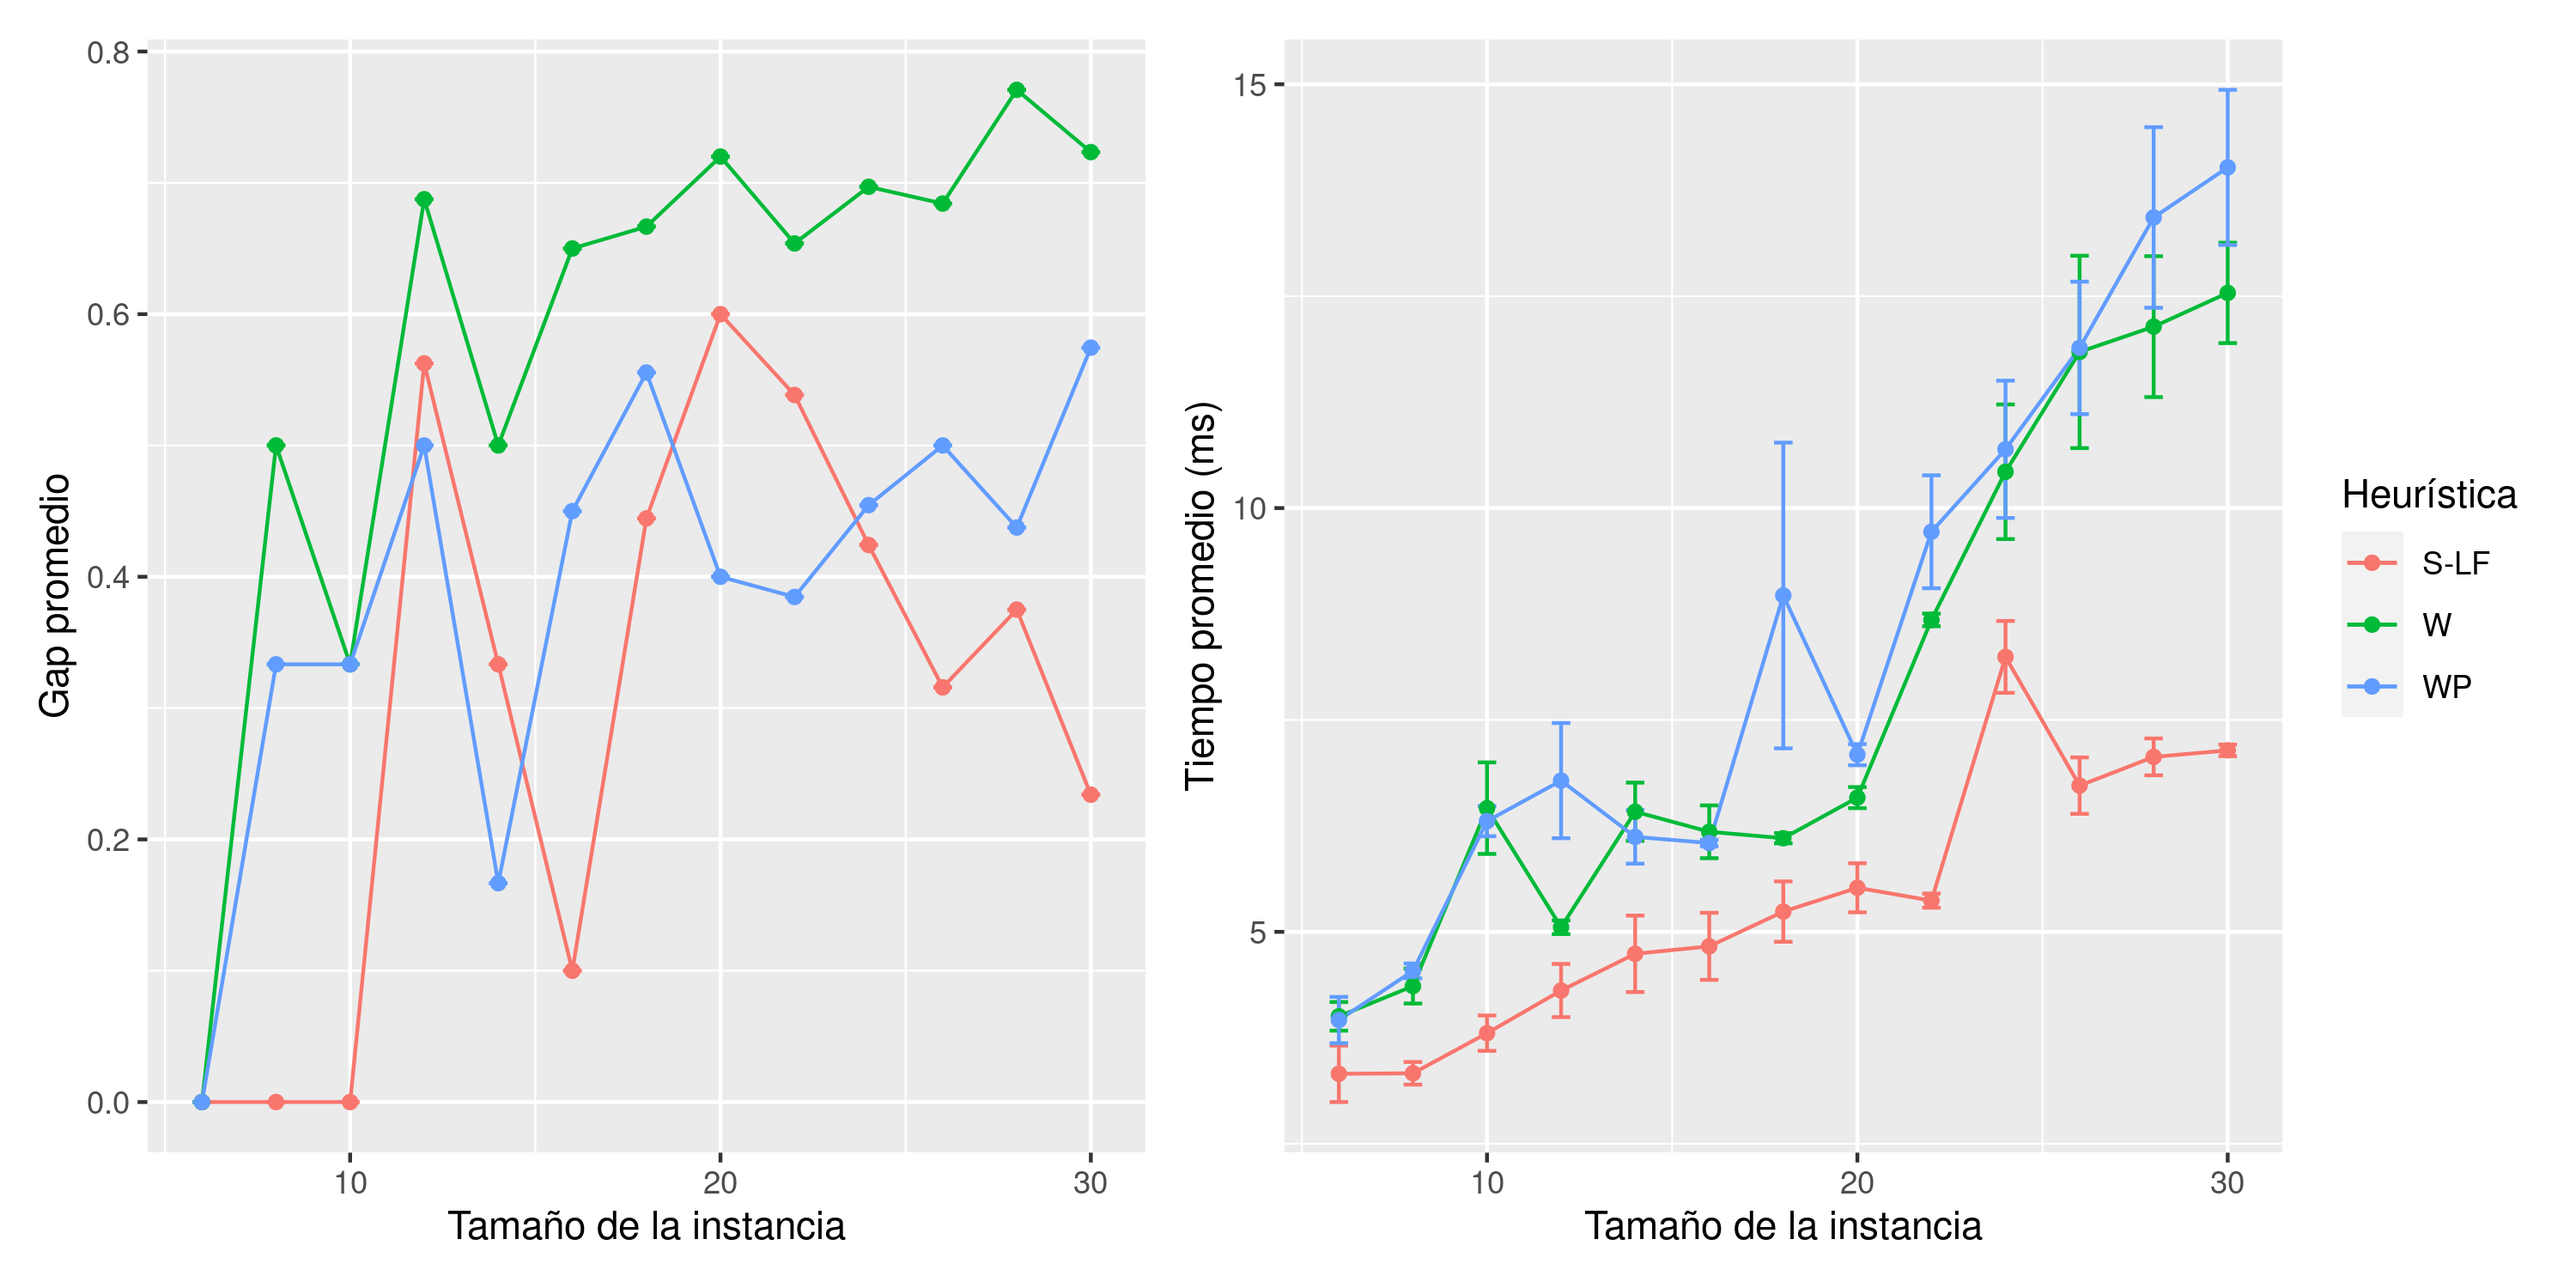
\includegraphics[width=.9\textwidth]{plots/heuristicas_constructivas.png}
    \caption{Gap relativo promedio en función del tamaño de la instancia (izq.) y tiempo promedio de ejecución en función del tamaño de la instancia. Los puntos representan el valor medio y las barras el error estándar. Se realizaron 5 repeticiones por instancia.}
    \label{plot:heuristicas constructivas}
\end{figure}

Por otro lado, también se observa que para muchas instancias el desempeño de WP y SL-F parece ser comparable. Sin embargo, para tamaños de instancia muy chicos y muy grandes S-LF parece ser mejor. Una posible explicación para las instancias de mayor tamaño es que como WP busca aumentar el impacto evaluando vértices de a pares, dependiendo del orden de evaluación de los vértices conectados en H, podría ocurrir que se generen subgrupos de vértices con colores distintos. Esto no pasaría en S-LF ya que minimiza la cantidad de colores, aumentando así el impacto como consecuencia y desconociendo las relaciones presentes en H. Finalmente, se puede observar que el tiempo de ejecución de SL-F es mucho menor al de las otras dos heurísticas constructivas golosas. 

\begin{figure}[H]
    \centering
    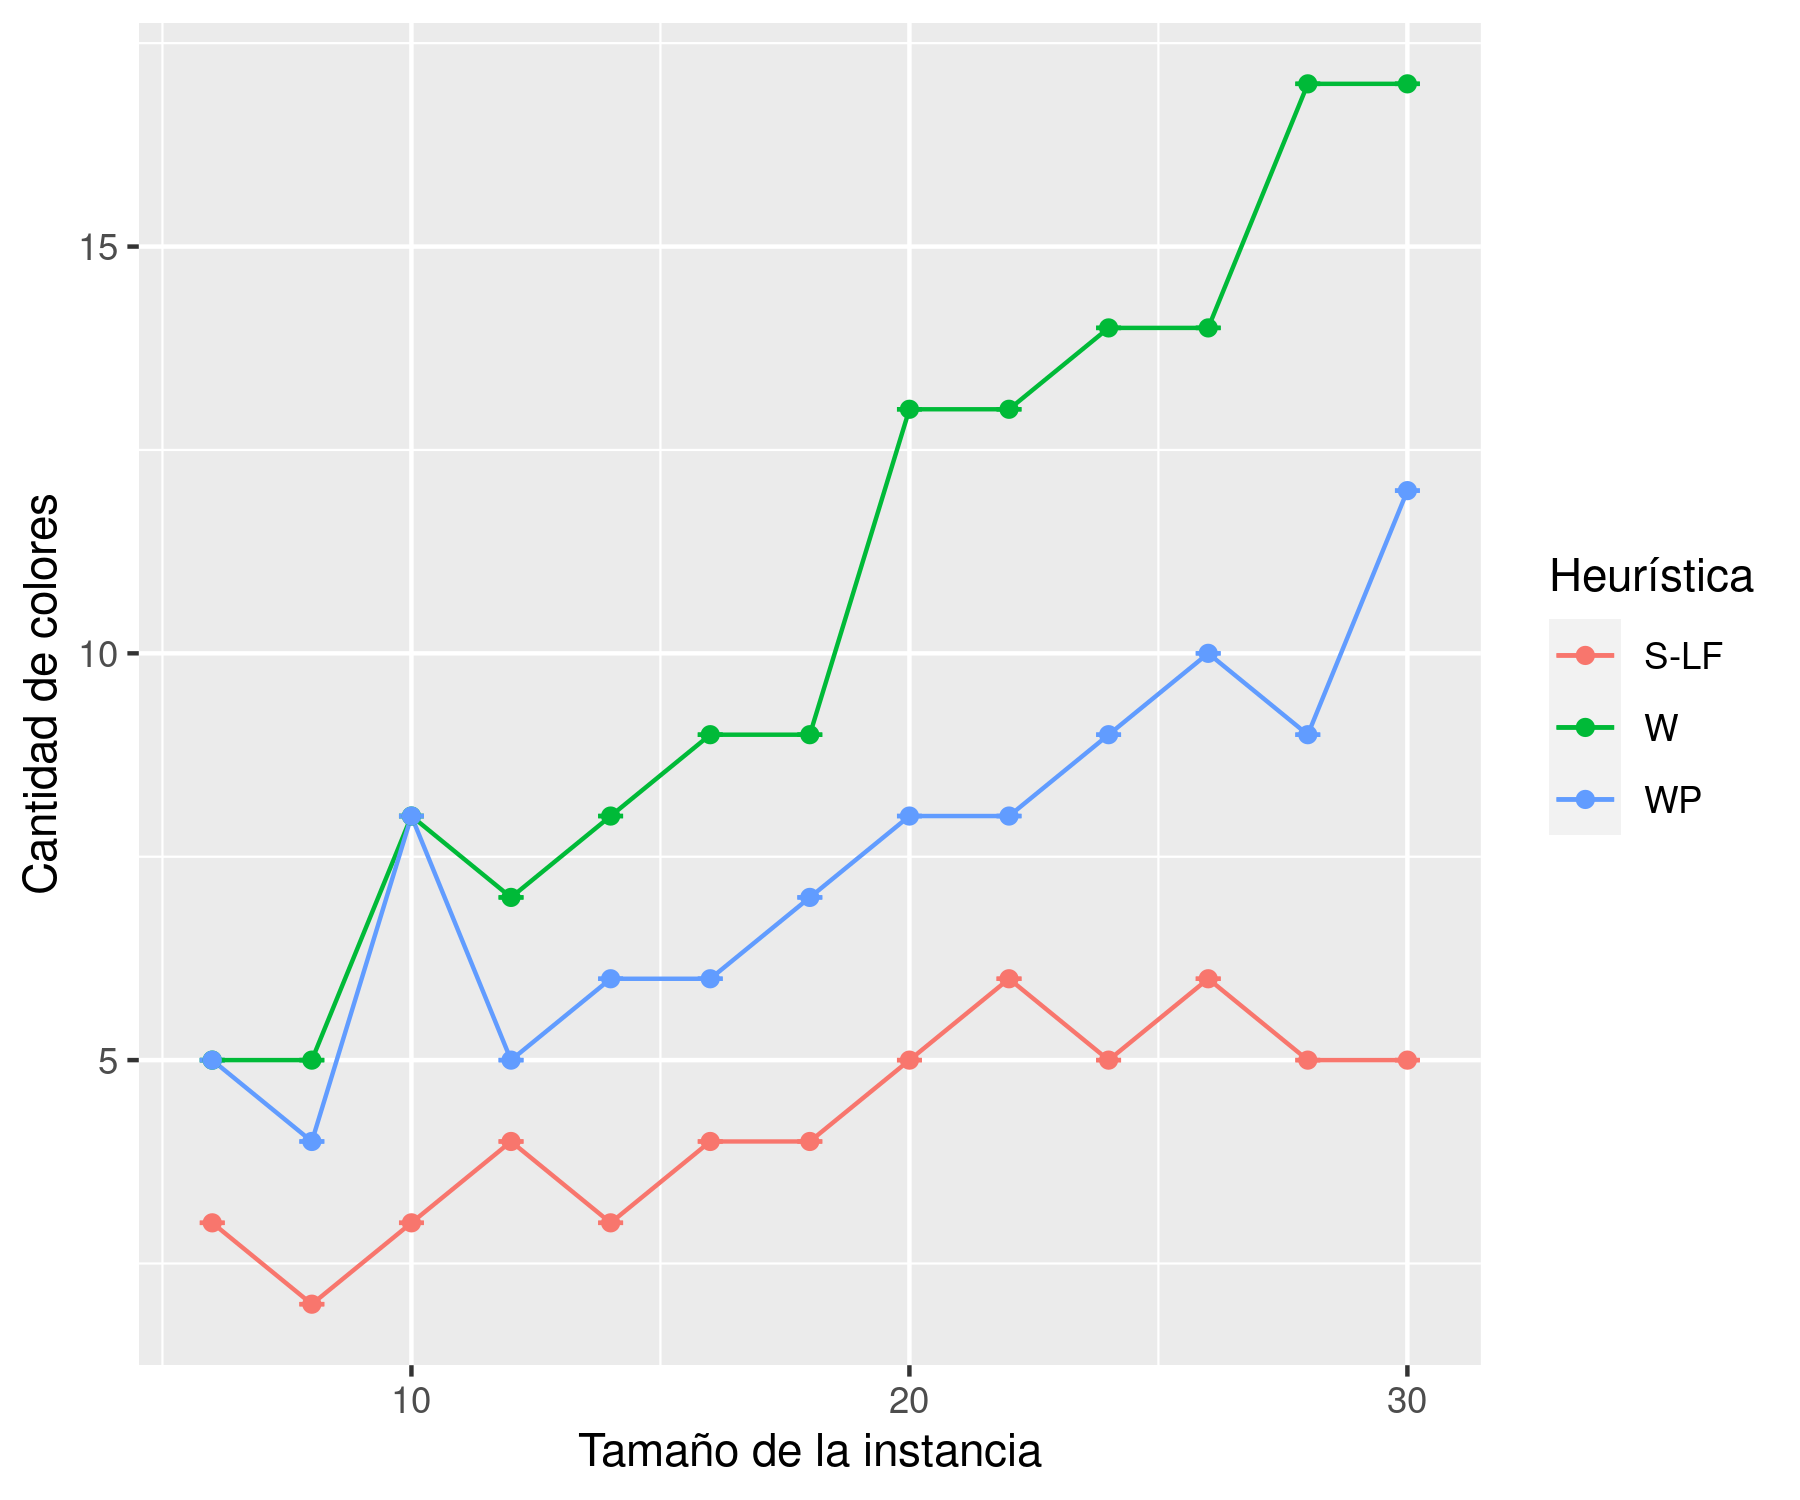
\includegraphics[width=0.6\textwidth]{plots/heuristicas_constructivas_colores.png}
    \caption{Cantidad de colores de la solución obtenida en función del tamaño de la instancia para las distintas heurísticas constructivas golosas. Se realizaron 5 repeticiones por instancia.}
    \label{plot:heuristicas constructivas colores}
\end{figure}

En la \cref{plot:heuristicas constructivas colores} se corrobora que, para cada tamaño de instancia, la cantidad de colores de la solución obtenida es mayor para W, intermedia para WP y menor para S-LF.

Teniendo en cuenta los resultados de esta sección, se concluye que S-LF es la mejor heurística constructiva golosa en términos de distancia respecto del óptimo y tiempo de ejecución. Sin embargo, esto no implica que necesariamente sea la mejor heurística inicial para todas las metaheurísticas y parámetros posibles porque la cantidad de coloreos de la solución inicial podría tener un impacto importante sobre la posibilidad de generar vecinos, dependiendo de la estrategia empleada por cada metaheurística.

\subsection{Impacto de parámetros}

De acuerdo a lo concluido en la sección anterior, se evaluó a cada metaheurística partiendo de la solución proporcionada por cada una de las heurísticas constructivas golosas. Adicionalmente, para cada una de estas combinaciones, se variaron los parámetros de las metaheurísticas como se describe en la sección \ref{section:metodologia-experimental} con el objetivo de poder encontrar una configuración óptima. Para esto sólo se utilizaron las instancias de entrenamiento.

\begin{figure}[H]
    \centering
\begin{subfigure}[b]{0.7\textwidth}
         \centering
         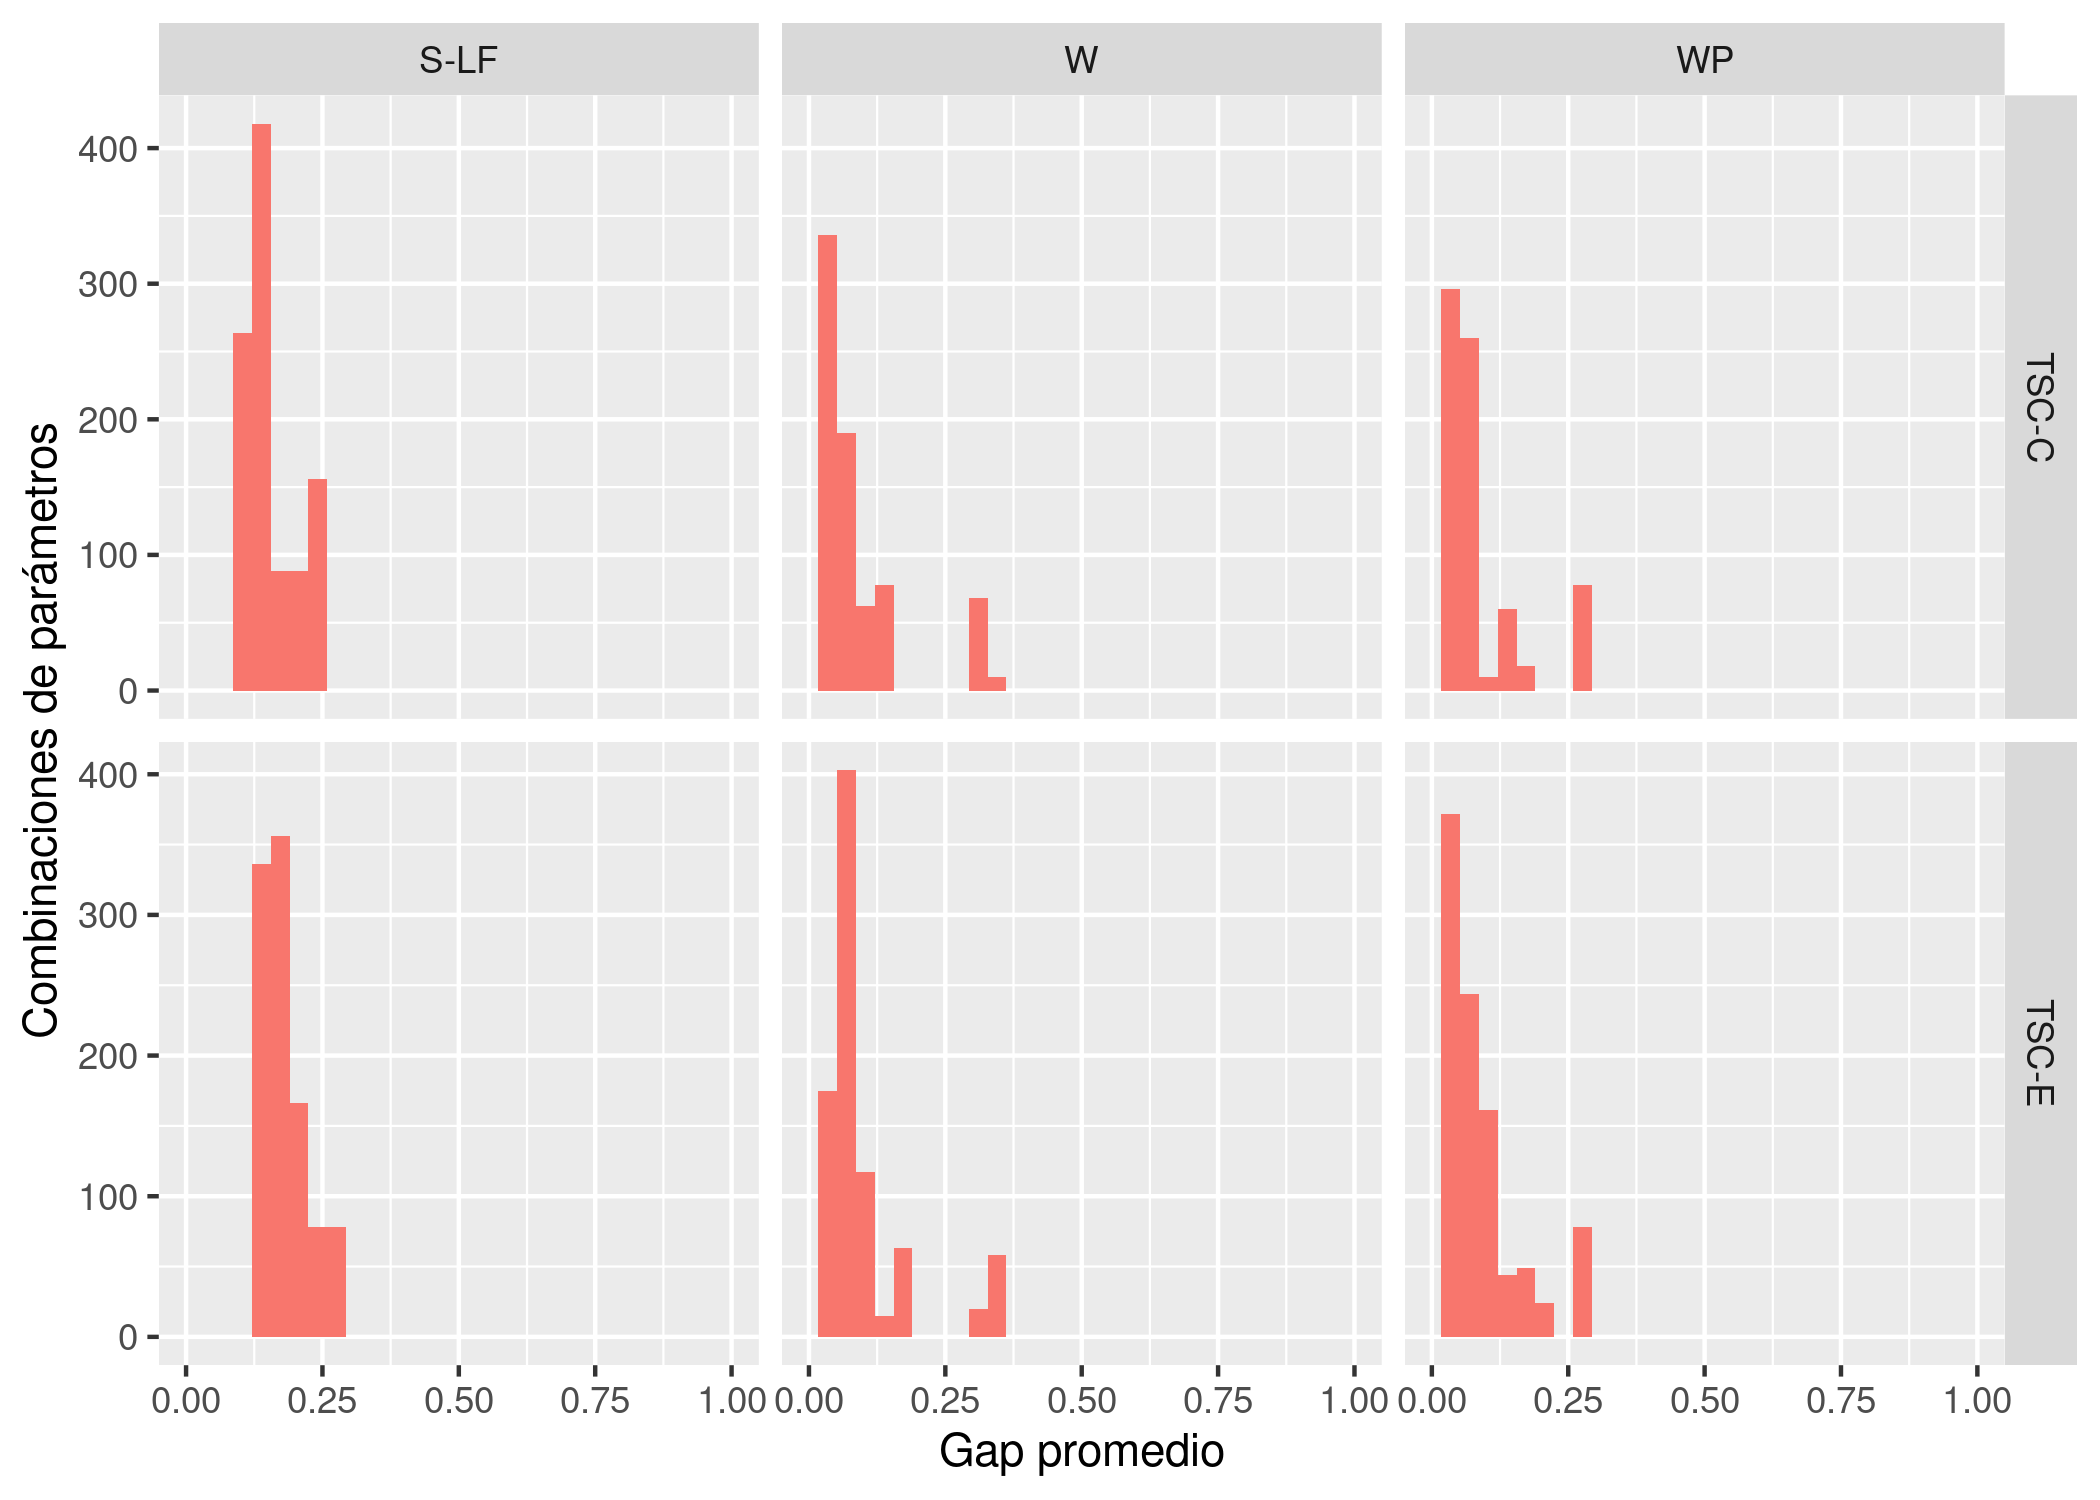
\includegraphics[width=\textwidth]{plots/histograma_tsc.png}
         \label{fig:histogramas-TSC}
\end{subfigure}
\begin{subfigure}[b]{0.7\textwidth}
         \centering
         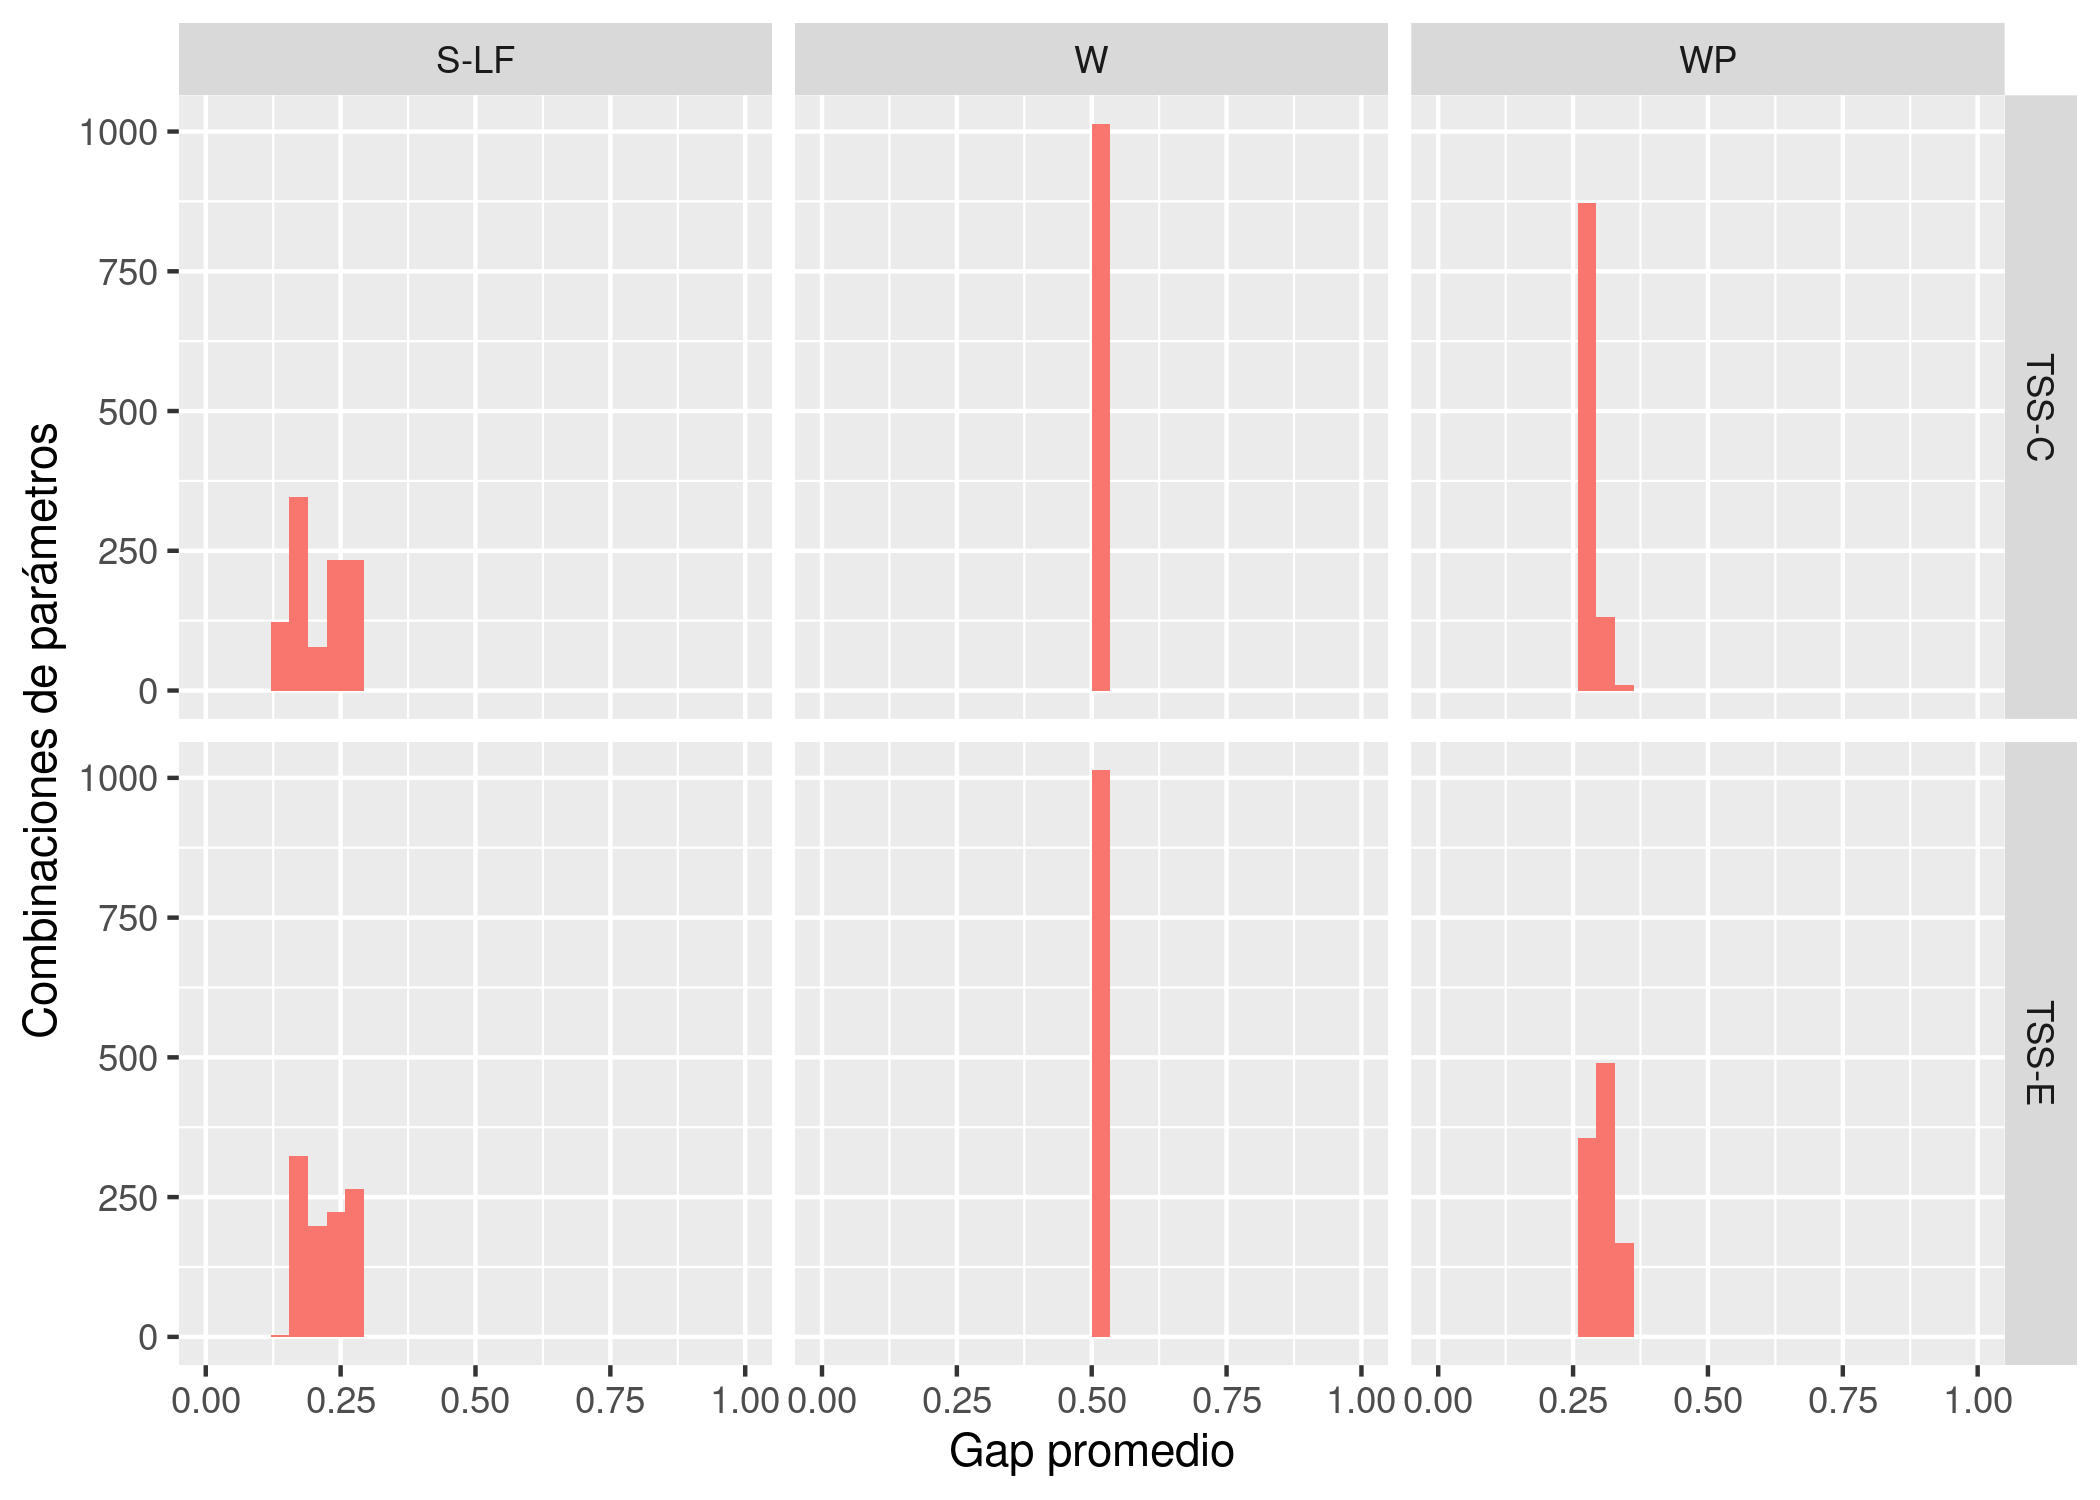
\includegraphics[width=\textwidth]{plots/histograma_tss.png}
         \label{fig:histogramas-TSS}
\end{subfigure}
\caption{Histogramas que indican la cantidad de combinaciones de parámetros que resultan en un mismo valor de gap relativo promedio. En la parte superior, se muestran los resultados obtenidos para las variaciones de Tabú search que usan vecindades generadas por la metodología \textbf{change} (TSC) y, en parte inferior, los resultados obtenidos para las variaciones que usan vecindades generadas por la metodología \textbf{swap} (TSS). A su vez, cada una está dividida en paneles según el tipo de memoria usada (C por coloreo y E por estructura) y la heurística constructiva inicial empleada (S-LF, W o WP).}
\label{plot:histogramas}
\end{figure}

En la \cref{plot:histogramas} se muestran, en la parte superior, los resultados obtenidos para las variaciones de Tabú search que usan vecindades generadas por la metodología \textbf{change} (TSC) y, en parte inferior, los resultados obtenidos para las variaciones que usan vecindades generadas por la metodología \textbf{swap} (TSS). A su vez, cada una está dividida en paneles según el tipo de memoria usada (C por coloreo y E por estructura) y la heurística constructiva inicial empleada (S-LF, W o WP). En cada panel se grafica un histograma que indica la cantidad de combinaciones de parámetros que resultan en un mismo valor de gap relativo promedio.

En líneas generales, a pesar de los amplios rangos de los parámetros evaluados, se observa una gran cantidad de combinaciones de los mismos que dan resultados equivalentes. En la siguientes secciones se intentará comprender por qué ocurre esto.

Más allá de esto, para TSC (figura superior) se observa un rango de variación en la calidad de la solución ocasionado por la variación de los parámetros independientemente del tipo de memoria y de la heurística constructiva inicial. Adicionalmente, para esta metodología de construcción de vecindad, parece ser peor la heurística constructiva S-LF que WP y W, ya que para estás últimas dos el mejor gap está más cerca de $0$. Sin embargo, existen combinaciones de parámetros que permiten obtener resultados comparables entre todos los tipos de heurísticas constructivas golosas para TSC.

En el caso de TSS (figura inferior) la variación en la calidad de la solución es más reducida y es dependiente de la heurística constructiva inicial. Se observan grandes diferencias de gap promedio que parecen depender más de la heurística inicial que de los parámetros. A pesar de esto, se puede concluir que, en el caso de emplear la heurística constructiva S-LF, parece haber lugar para la optimización de parámetros y posiblemente en el caso de WP también. Para esta metodología de generación de vecinos, parece ser mejor la heurística S-LF que W y WP ya que el mejor $gap$ está más cerca de 0 para S-LF. Adicionalmente, no existe combinación de parámetros que logre resultados competitivos para W y WP respecto de S-LF.

Para analizar el impacto de variar cada parámetro sobre el desempeño de las metaheurísticas y tratar de comprender por qué distintas combinaciones de los mismos pueden resultar equivalentes, se decidió empezar evaluando el efecto de variar el porcentaje de vecindad.

\subsection{Impacto del porcentaje de vecindad}

Dados los resultados vistos en la sección anterior, resultó interesante comenzar a analizar cada parámetro en particular para intentar dilucidar el impacto de cada uno en el desempeño de los algoritmos. Se comenzó analizando el efecto de tomar distintos tamaños de vecindad, ya que esto podría implicar cambios notables en el comportamiento del algoritmo. Para tamaños de vecindad baja, podría suceder que se ignoren mejoras de impacto que formen parte de la vecindad pero hayan quedado fuera por estar tomando una porción demasiado pequeña. Por el contrario, tomar la totalidad de la vecindad podría resultar en un estancamiento en óptimos locales.

En la \cref{plot:porcentaje vecindad} se puede observar una fuerte variación en los resultados al variar el porcentaje de vecindad. Respecto a TSC se puede ver que tomar una vecindad más grande resulta más provechoso, encontrando sus óptimos en los valores del rango $70 - 100$. Por el contrario, tomar una vecindad demasiado pequeña parece restringir demasiado las posibilidades de movimiento, inhabilitando posibles soluciones vecinas mejores.

Respecto de TSS se puede observar que algunos algoritmos como TSS-C-WP y TSS-E-WP encuentran óptimos para porcentajes de vecindad medianos. Se corrobora que TSS sólo varía el gap promedio de forma relevante cuando la heurística inicial es S-LF. Para la heurística WP la variación es mucho menor y para W es inexistente. Esto lleva a pensar junto con lo visto en la subfig. \ref{fig:histogramas-TSS}, que los algoritmos de \textit{Tabú Search Swap} no ofrecen mejoría alguna para el algoritmo inicial W, estancándose siempre en el impacto obtenido por la solución inicial. Sólo ofrecen mejoras leves para el algoritmo inicial WP.
 
Lo observado en esta sección permite concluir que el cambio del porcentaje de vecindad puede explicar en gran medida la variación del gap vista en la fig. \ref{plot:histogramas}, mostrando así la injerencia de este parámetro en la calidad de las soluciones obtenidas por el algoritmo. Por este motivo, se decidió evaluar el impacto de los parámetros restantes teniendo en cuenta el porcentaje de vecindad empleado.

\begin{figure}[H]
    \centering
    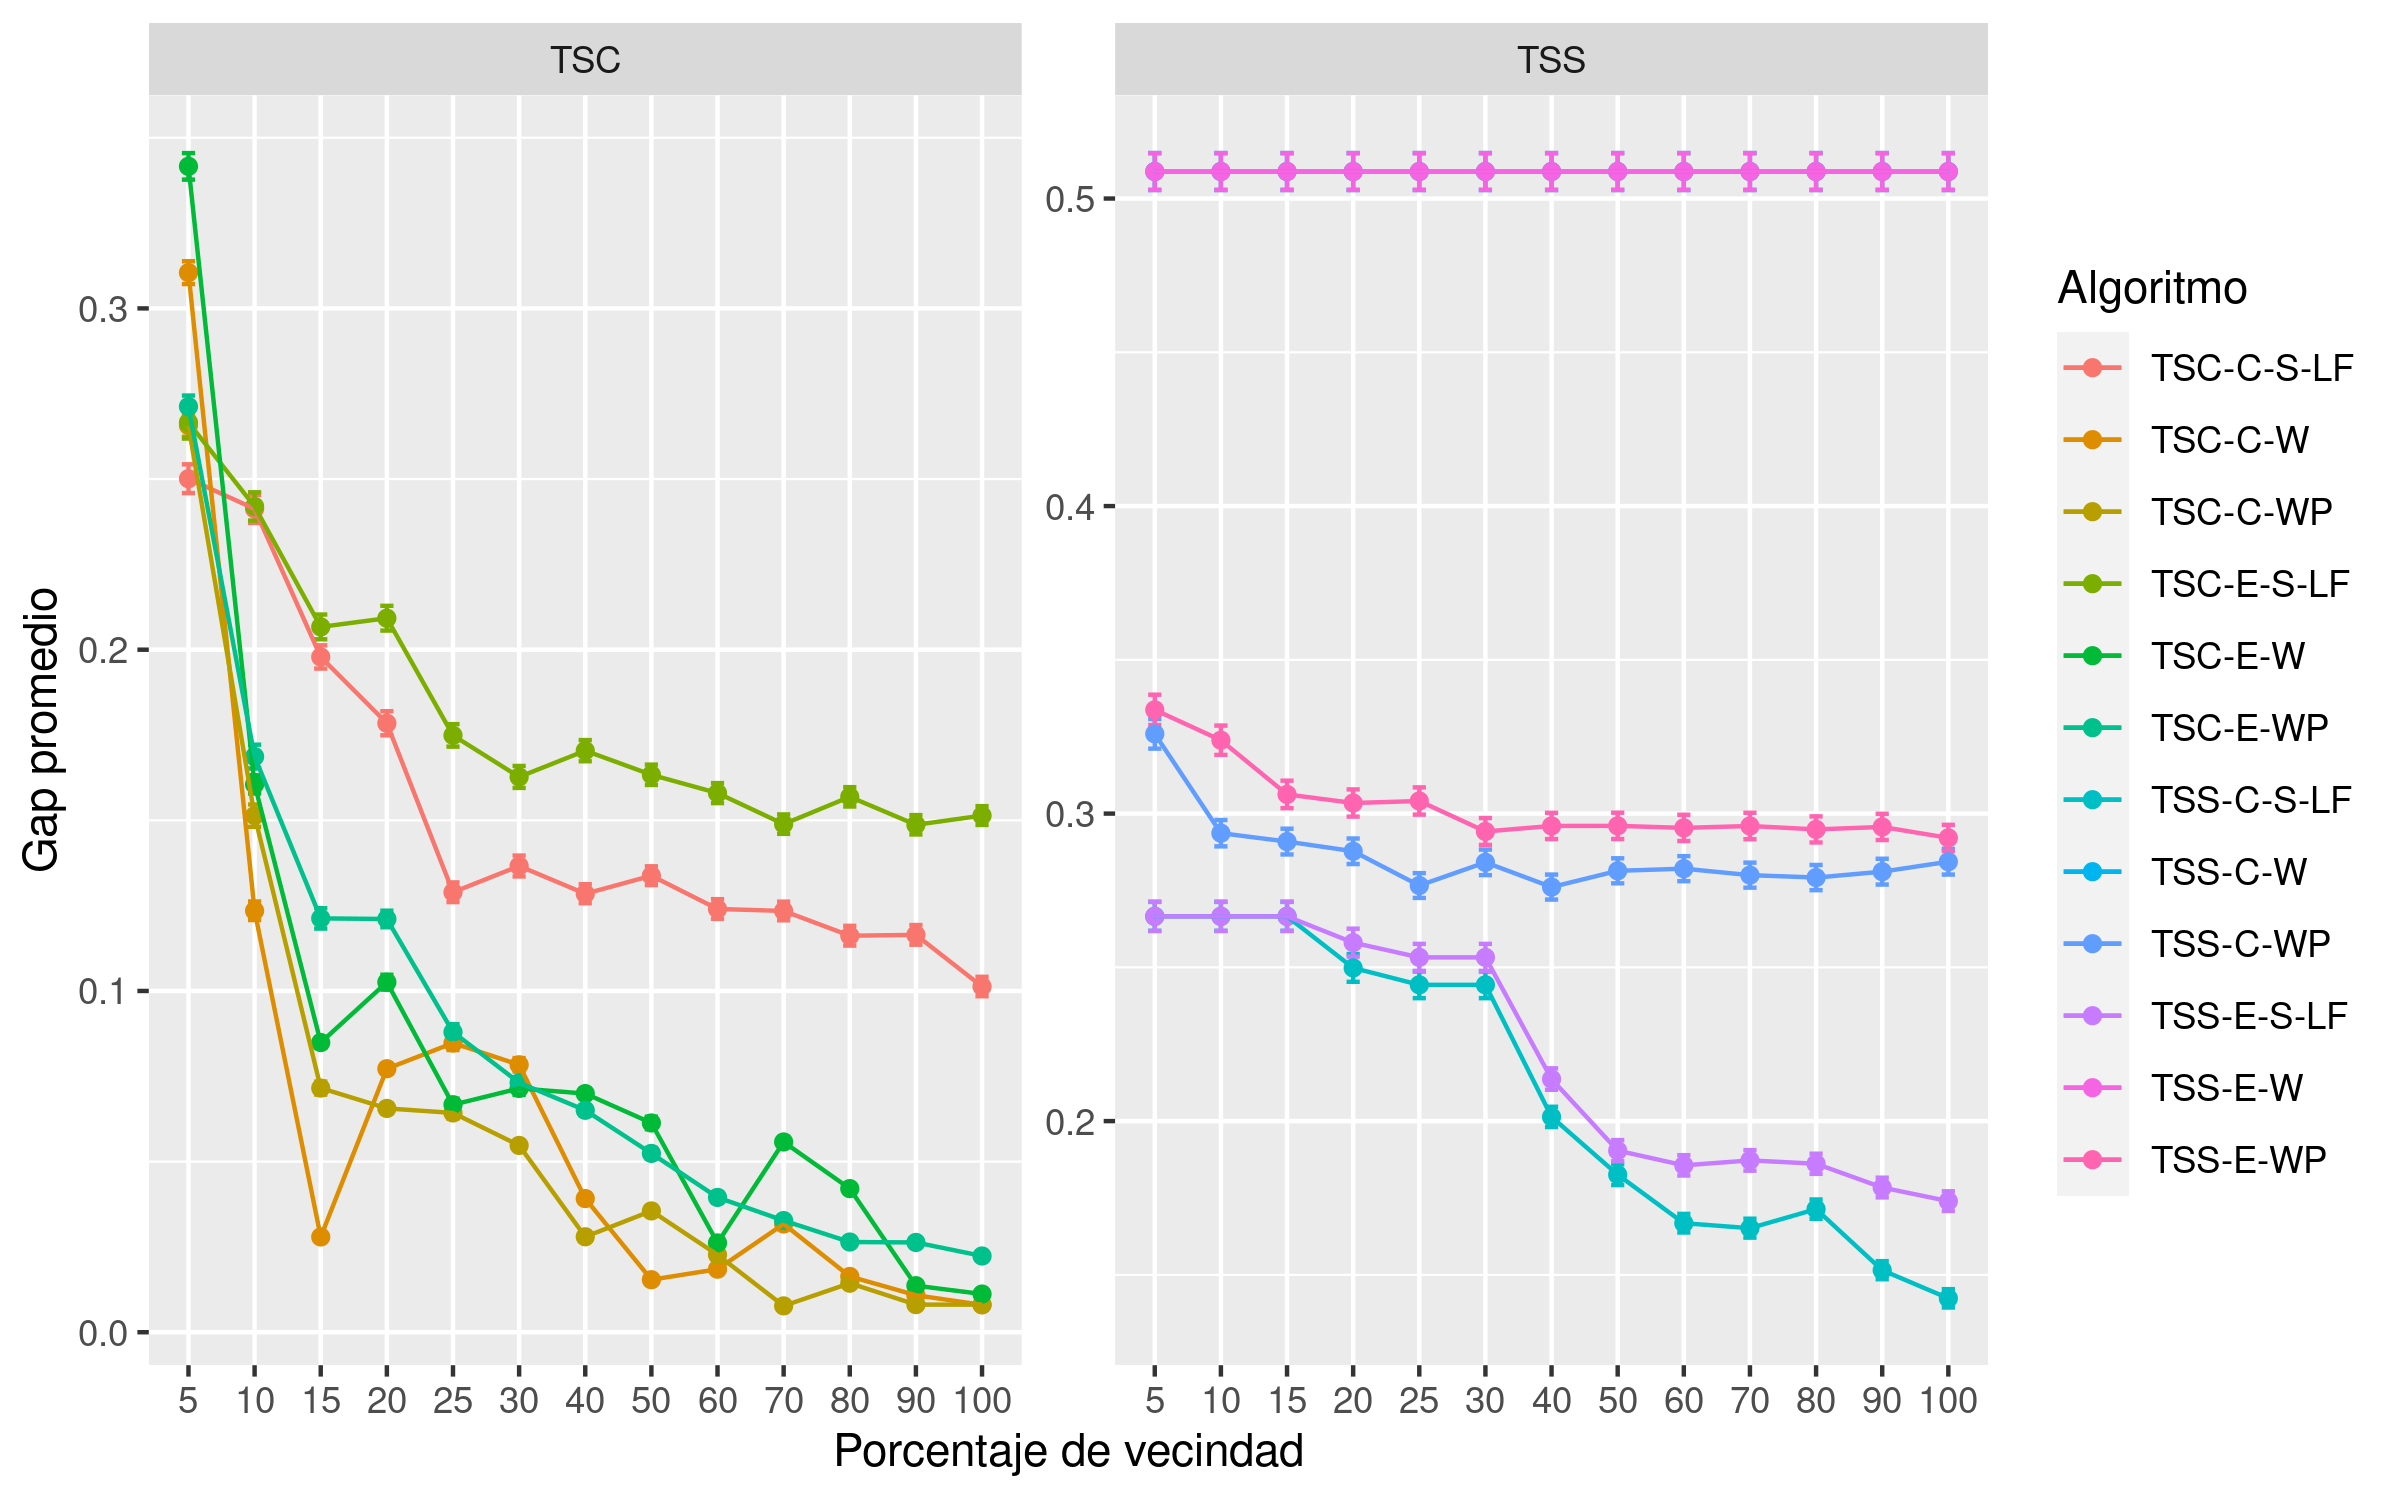
\includegraphics[width=0.8\textwidth]{plots/porcentaje_vecindad.png}
    \caption{{Gap promedio según combinación de algoritmo de Tabú Search con algoritmo goloso inicial para diferentes porcentajes de vecindad.}}
    \label{plot:porcentaje vecindad}
\end{figure}

\subsection{Impacto de aspirar}

Otro de los metaparámetros cuyo análisis resultó importante fue la utilización de una función de aspiración. Para ello, se corrieron los diferentes métodos de Tabú con un algoritmo goloso inicial óptimo para cada uno. Los resultados de TSS no presentaron diferencia alguna en la utilización de la función de aspiración para ninguna estructura de memoria.

\begin{figure}[H]
    \centering
    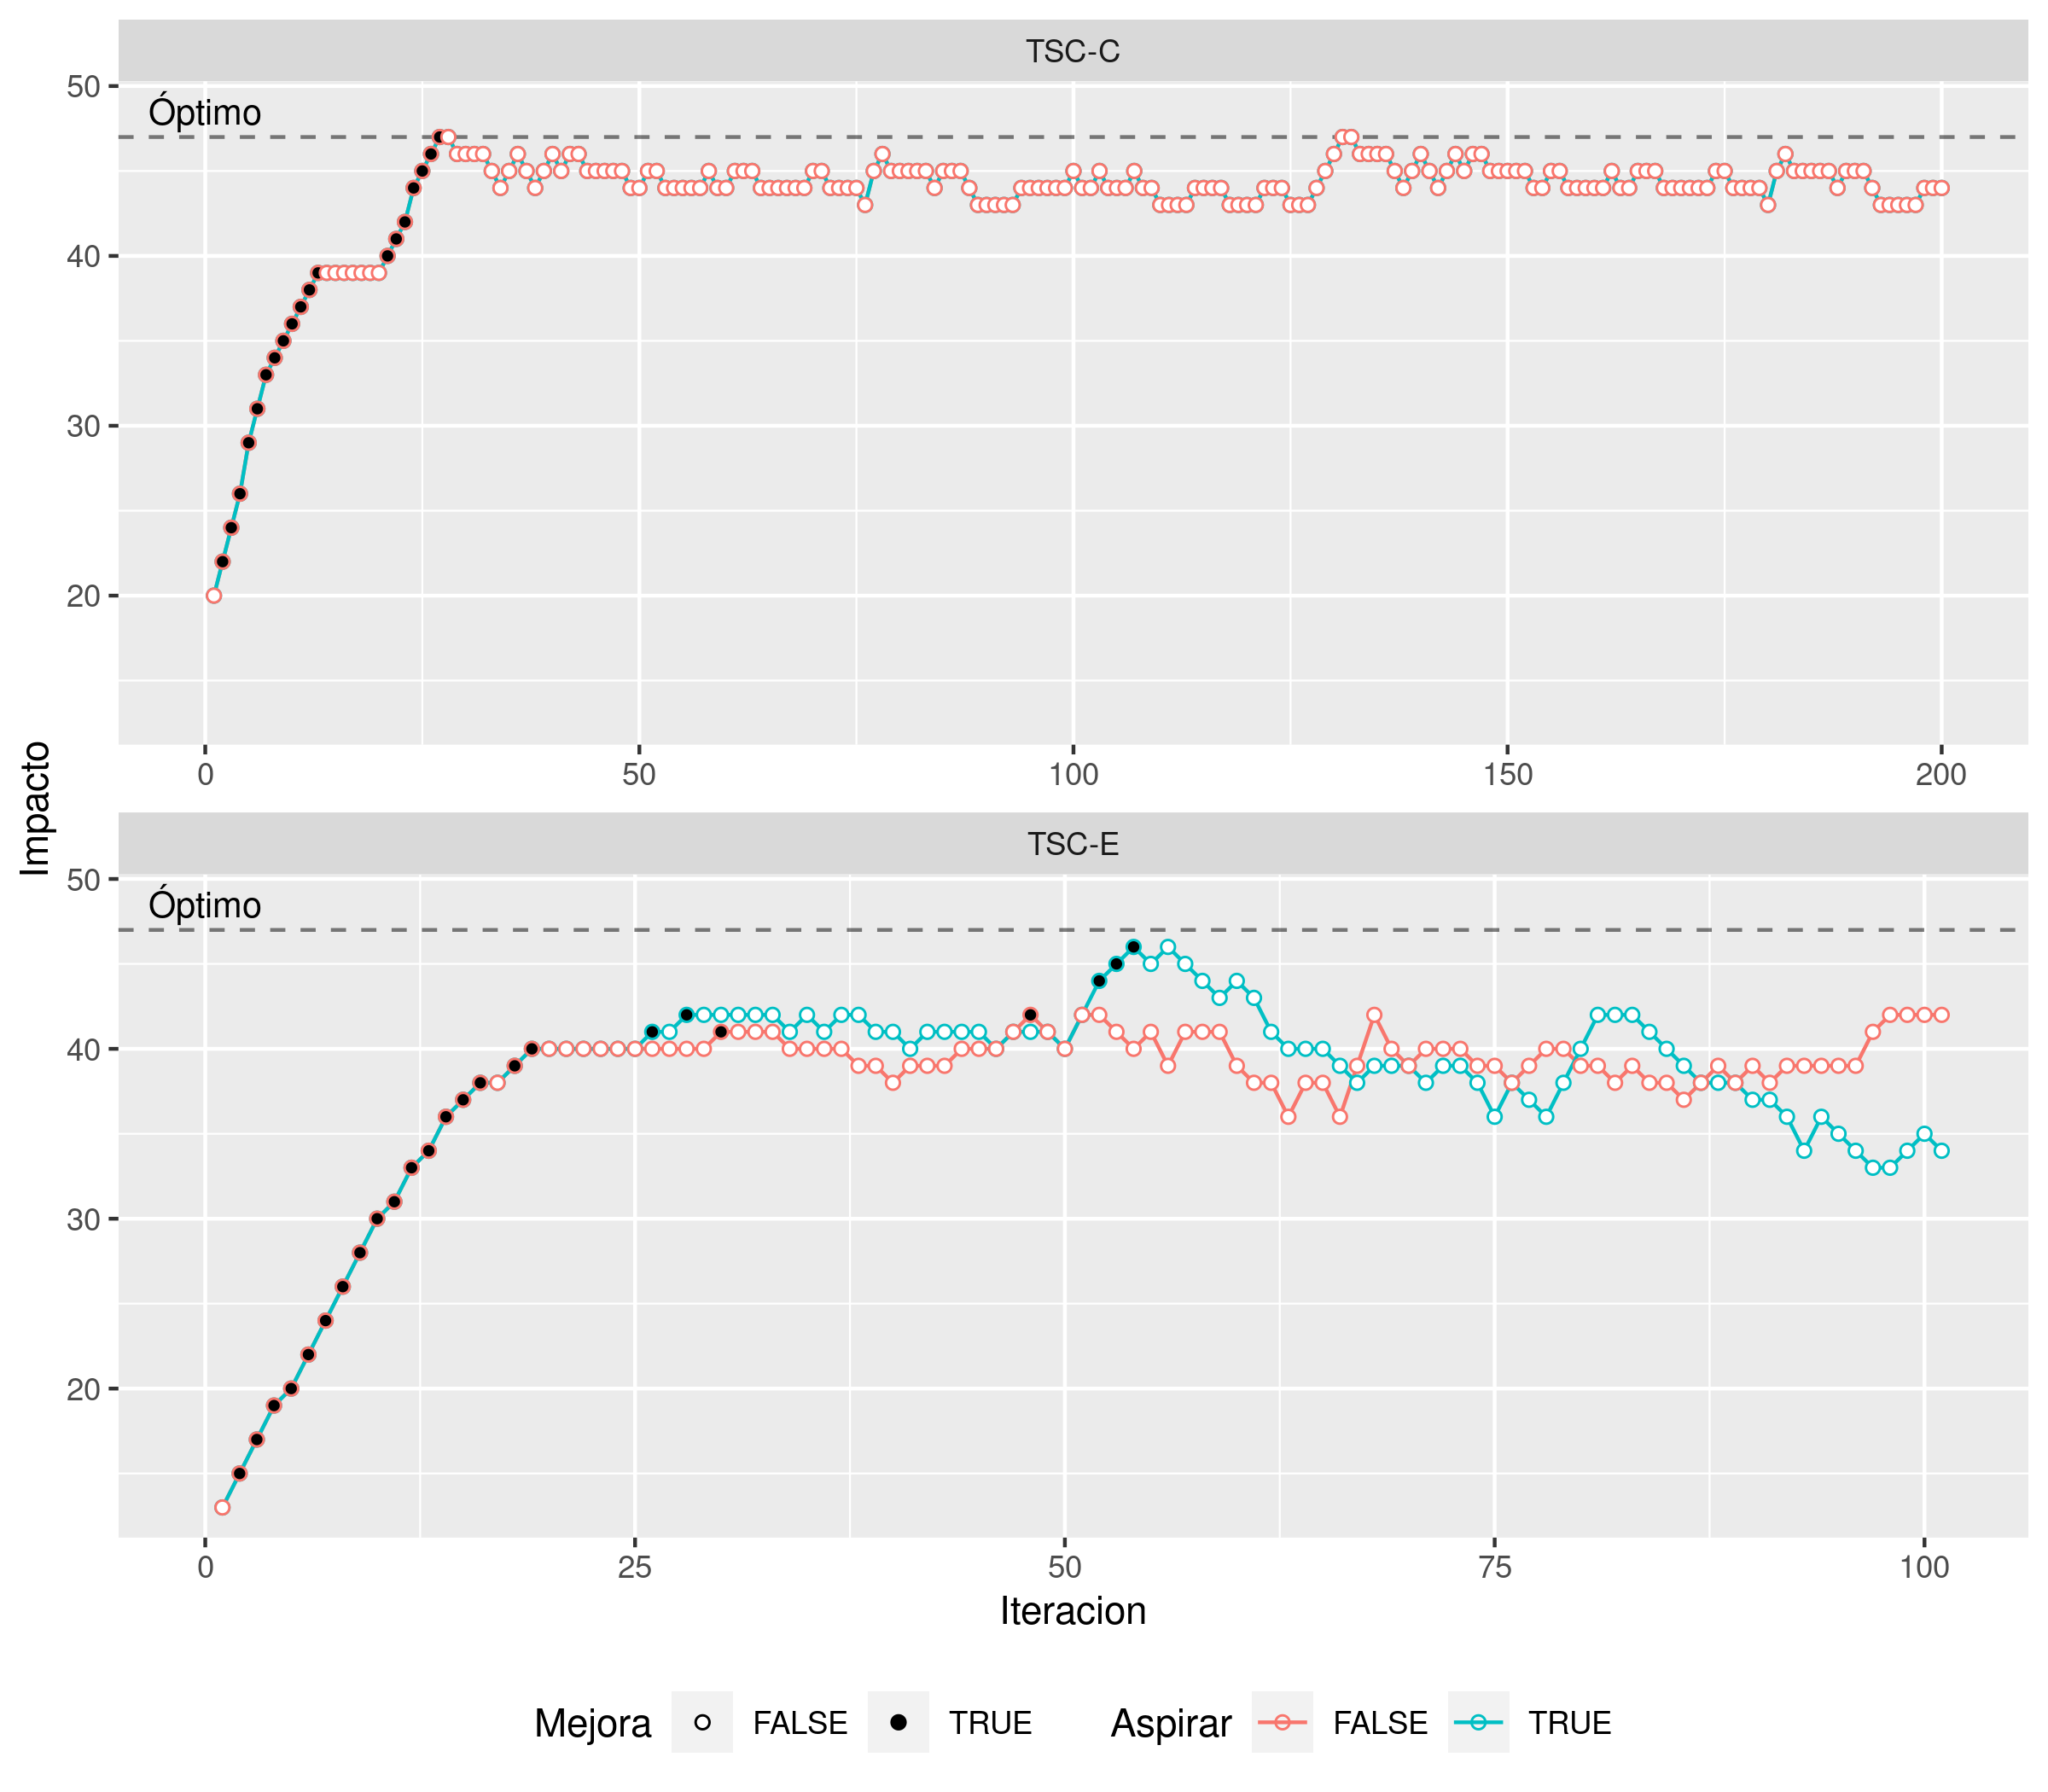
\includegraphics[width=0.7\textwidth]{plots/impacto_tiempo.png}
    \caption{Se observa el impacto en función del número de iteraciones para los algoritmos TSC-C Y TSC-E. Se observan en rojo los casos evaluados con función de aspiración y, en azul, aquellos que no. Los círculos rellenos implican que se observa una mejora en el impacto. Se realizaron 5 repeticiones por instancia.}
    \label{plot:impacto vs iteracion}
\end{figure}

Para el algoritmo TSC se observan dos situaciones diferentes. En el caso de utilizar una memoria por estructura se pueden obtener mejores resultados a partir de la función de aspiración. Esto se debe a que volver a utilizar un cambio de color en un vértice específico en un futuro coloreo distinto puede permitir una mejoría en el impacto de la solución, ya que dos coloreos radicalmente distintos (y con distinto impacto) pueden ser vecinos del mismo cambio estructural. En este sentido, la utilización de la función de aspiración permite desbloquear muchas soluciones posibles que permiten impactos distintos.

En el caso de utilizar una memoria por coloreo, aspirar no presenta ninguna diferencia con no hacerlo. Esto se condice con lo dicho anteriormente, ya que al haber pasado por un coloreo específico, se contemplan esa solución y sus vecinas. Luego, volver a pasar por esa situación no presenta nuevas oportunidades de coloreo que permitan una mejoría en el impacto. A su vez, resulta muy poco probable que un coloreo sufra los suficientes cambios como para pasar por una solución y luego volver exactamente al mismo coloreo. En este sentido, la probabilidad de volver a un coloreo exacto anterior resulta muy baja y no presenta ninguna mejoría, por lo que la función de aspiración no genera cambios en el impacto obtenido por esta implementación.

Finalmente, considerando la mejoría que brinda la función de aspiración, el costo temporal que ésta requiere resulta tolerable, por lo que resulta provechoso utilizarla. Esto puede verse en mayor profundidad en las figuras \ref{plot:aspirar tiempo tsc}, \ref{plot:aspirar tiempo tss}, \ref{plot:aspirar tsc} y \ref{plot:aspirar tss}.
 
\subsection{Impacto de tamaño de memoria}

En el paradigma computacional, los recursos de memoria y tiempo suelen ser elementos cuya optimización puede llevar a resultados considerablemente mejores. En el caso de los algorítmos metaheurísticos, la memoria y el tiempo resultan de vital importancia para un correcto funcionamiento. Sin embargo, se debe evitar el abuso de los mismos para no sumar gastos innecesarios. Por ello, se decidió establecer un rango amplio de memoria \ref{metodologia} y luego verificar cuánta era realmente necesaria para llegar a una buena solución.

Se corrió cada combinación de algoritmos Tabú con heurísticos iniciales y se graficó cada uno según porcentaje de vecindad. A su vez, se agregó una línea vertical con la cantidad de iteraciones efectivas\footnote{Iteraciones realmente efectuadas que terminaron antes de llegar al tope de iteraciones asignadas al algoritmo.} realizadas y sus respectivas barras de error, lo que permitió analizar en detalle la real utilización de la memoria.

\begin{figure}[H]
    \centering
    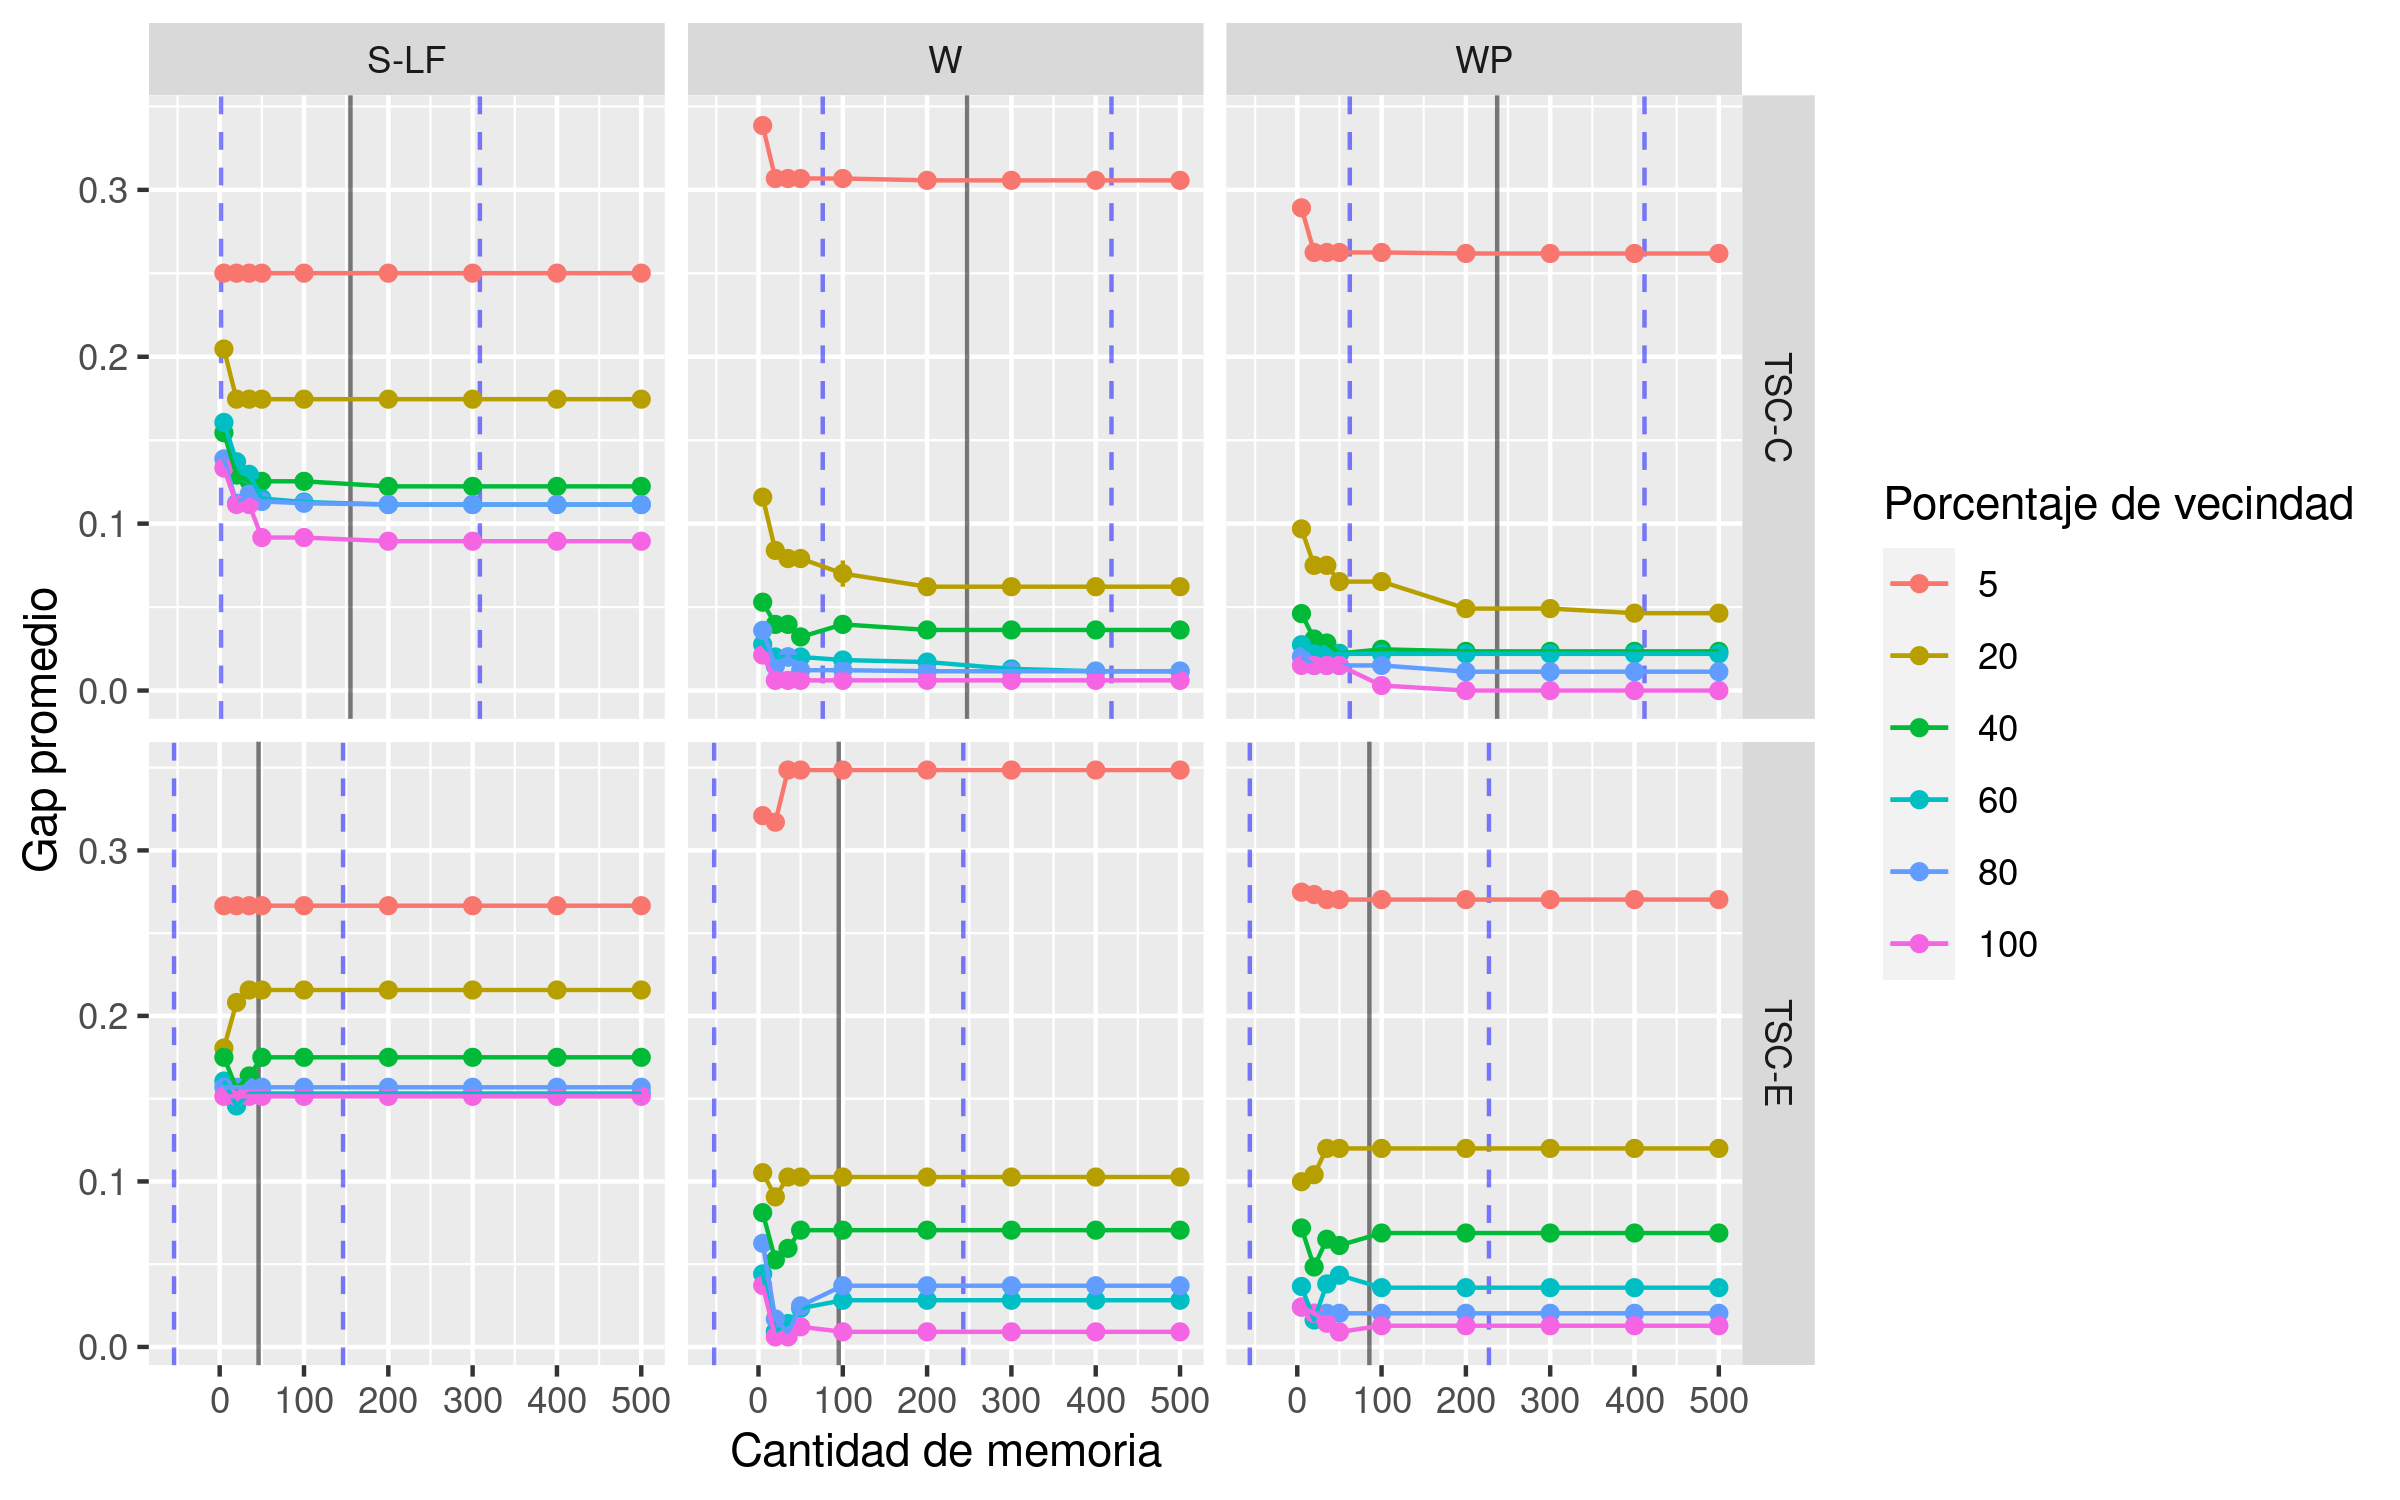
\includegraphics[width=0.8\textwidth]{plots/memoria_tsc.png}
    \caption{Gap promedio según cantidad de memoria asignada para cada combinación de algoritmo. Se grafican líneas verticales con iteraciones efectivas realizadas por cada algoritmo.}
    \label{plot:memoria tsc}
\end{figure}

En el caso de TSC, se puede observar que las iteraciones efectivas hacen que memoria no se use, lo que indica que no hace falta tanta memoria en algunos algoritmos. A su vez, no se notan cambios significativos en el gap para memoria mayor a 200 aproximadamente, lo que parecería mostrar que no es necesaria una gran cantidad de memoria para mantener una zona tabú efectiva.

A su vez, entre las dos diferentes estructuras de TSC (TSC-E y TSC-C) se ven diferencias en las iteraciones efectivas, realizando TSC casi el doble en promedio.  Esto podría deberse a lo explicado anteriormente, ya que al no recortar tanto la vecindad por la zona tabú definida en base a coloreo, se precisan más iteraciones para analizar la vecindad hasta quedarse sin vecinos o terminarse las iteraciones.

Respecto a los algoritmos iniciales elegidos, se puede observar que W y WP funcionan de manera similar en TSC-C y TSC-E pero S-LF no. Esto se debe a que la lógica del \textit{change} genera un nuevo vecino a partir de colores pre-existentes en el grafo no presentes en sus adyacentes. Por lo tanto, sólo puede mantener o disminuir el número de colores en el grafo. En consecuencia, al partir de una heurística golosa que minimiza la cantidad de colores\footnote{Notar que minimizar la cantidad de colores pensando únicamente en G puede ser contraproducente porque tener impacto implica repetir colores en H.}, la cantidad de soluciones posibles que puede explorar el algoritmo se ve reducida afectando negativamente a su performance.

\begin{figure}[H]
    \centering
    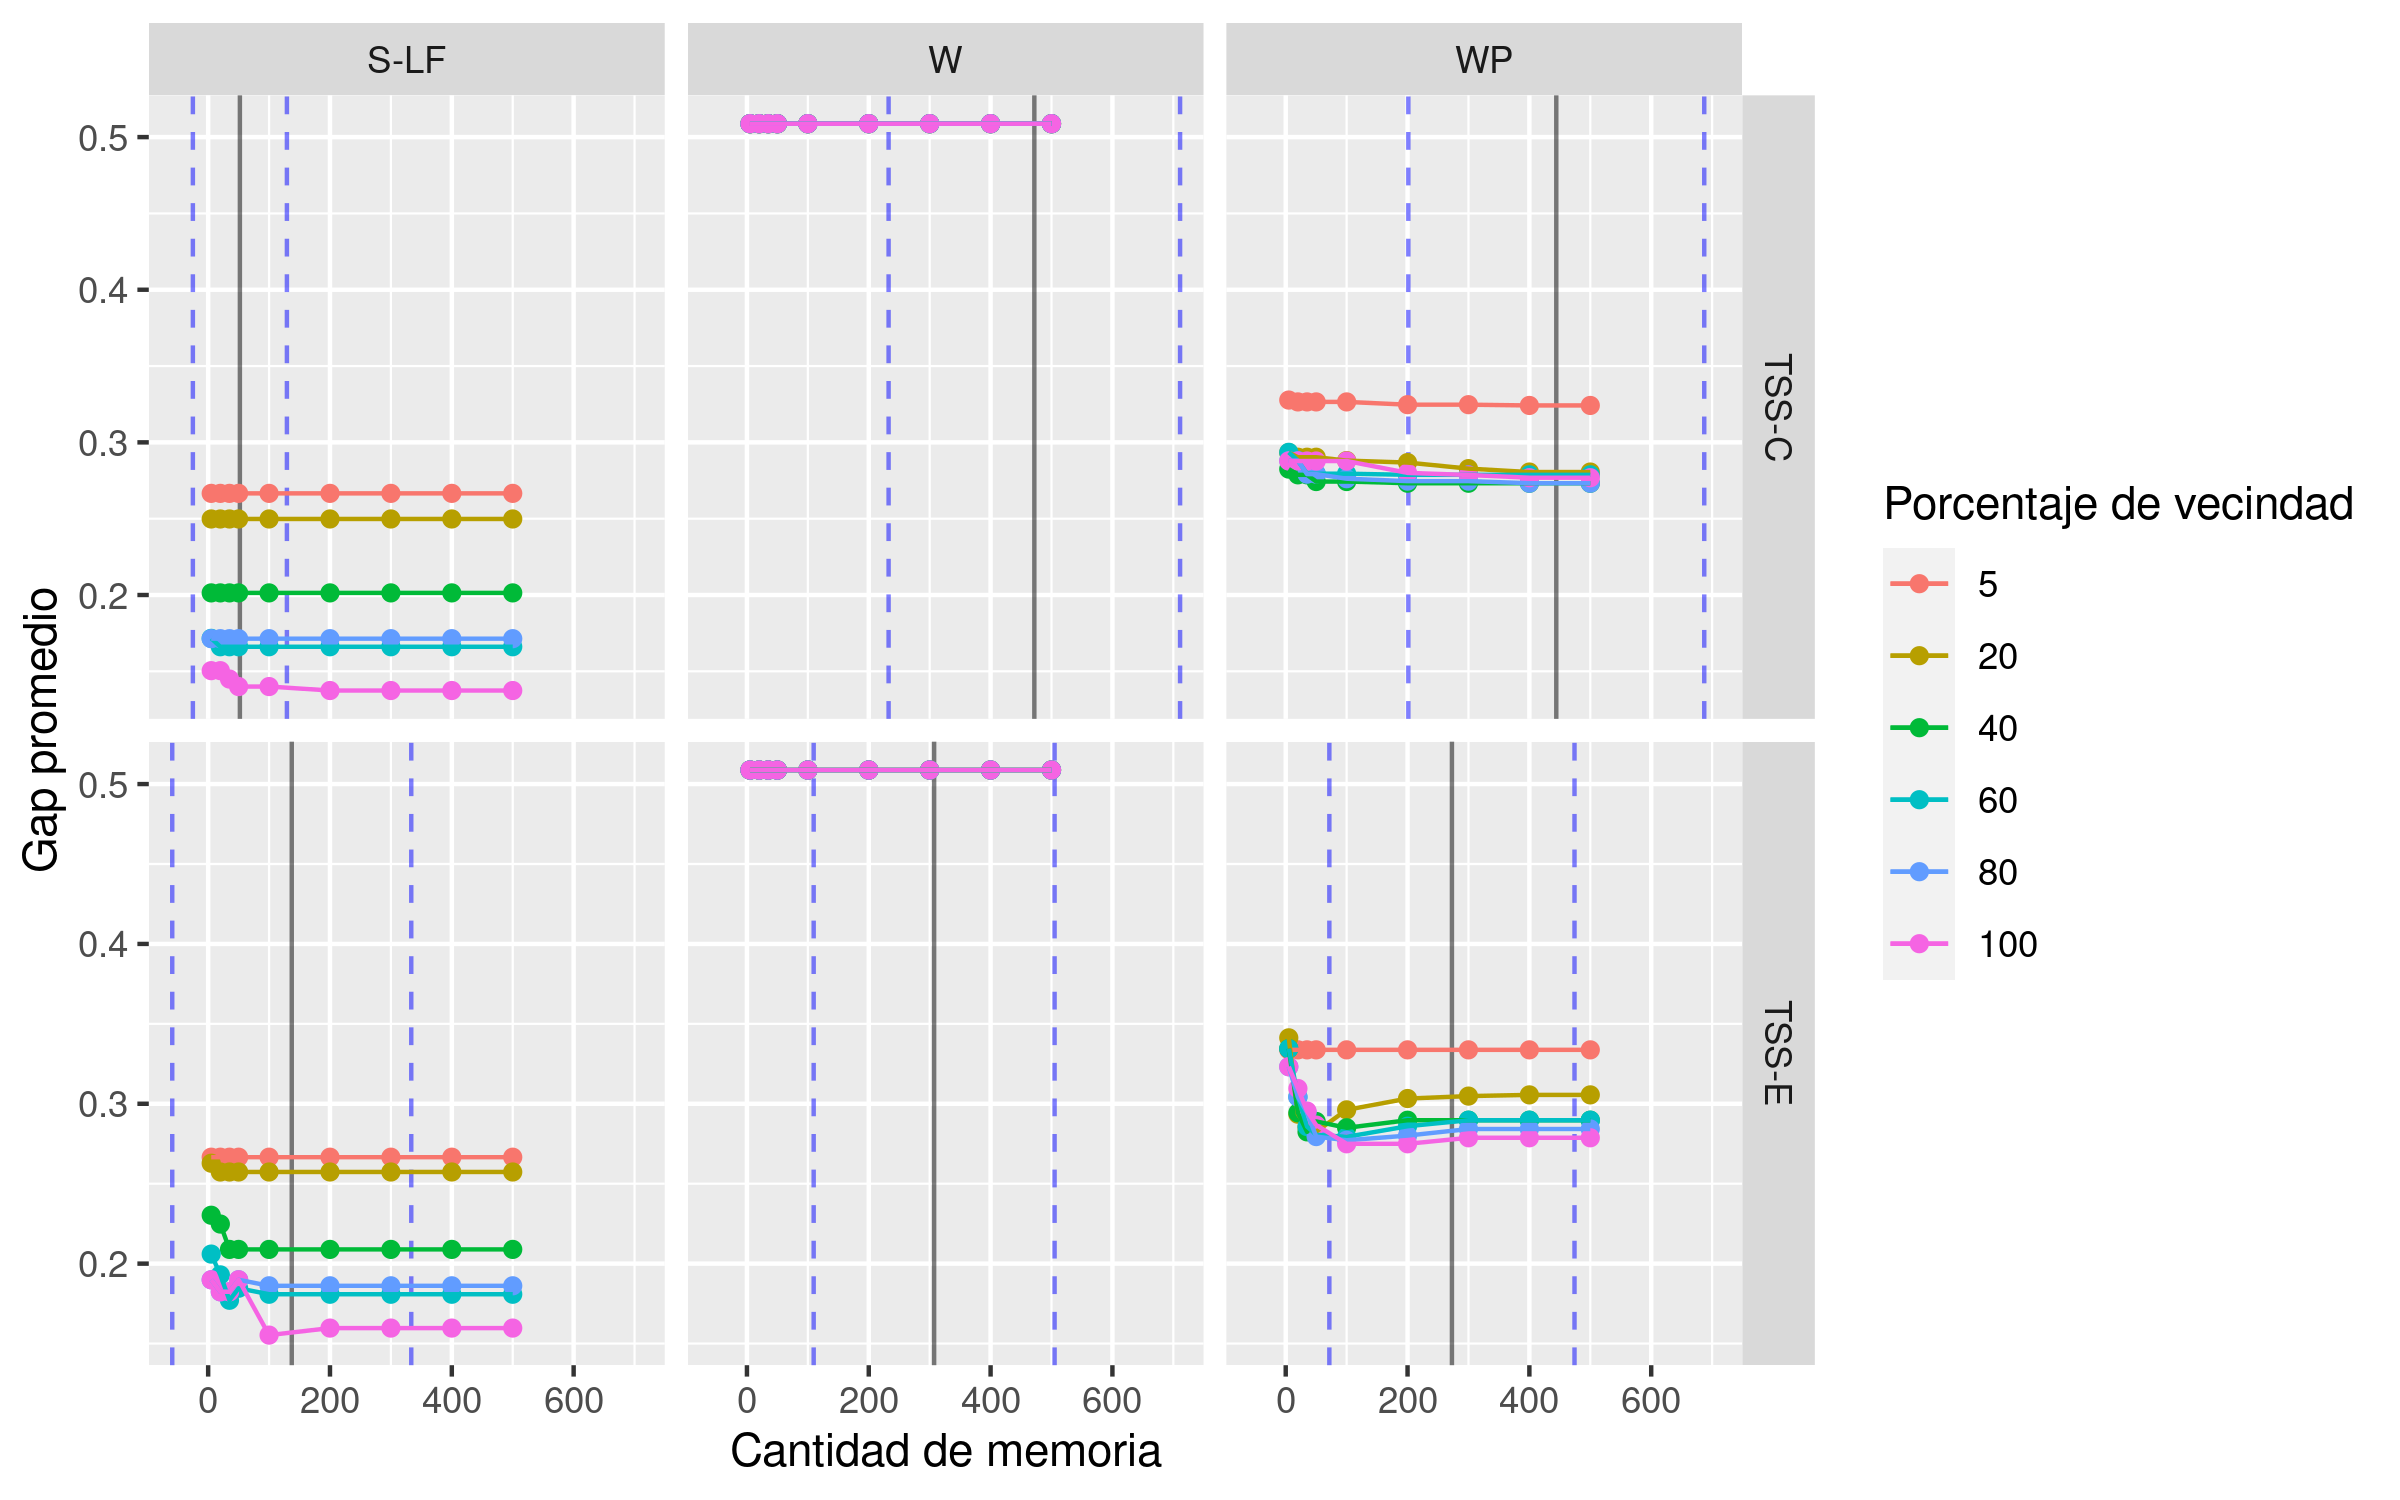
\includegraphics[width=0.8\textwidth]{plots/memoria_tss.png}
    \caption{Se observa el gap promedio en función de la cantidad de memoria para todas las combinaciones de tabú search swap y los algoritmos heurísticos iniciales. En todos los casos, se grafican los resultados obtenidos para valores de porcentaje de vecindad en [5, 20, 40, 60, 80, 100]. Se realizaron 5 repeticiones por instancia.}
    \label{plot:memoria tss}
\end{figure}

A primera vista, para TSS utilizando los algoritmos iniciales W y WP parecería tener sentido usar una gran cantidad de memoria, ya que no estaría siendo anulada por la cantidad de iteraciones. Sin embargo, para W la performance no cambia respecto de este parámetro, descartando esta posibilidad. En este caso, lo que sucede es que hay gran vecindad que la memoria no es capaz de cubrir completamente, por lo que siempre habrá vecinos para analizar (aunque no mejoren el impacto). Esto sucede porque la heurística golosa W utiliza muchos colores. Luego, como TSS sólo intercambia colores (no introduce nuevos) de vértices y W utiliza muchos colores, la vecindad resulta muy grande y la memoria no logra acapararla toda, por lo que el algoritmo prácticamente se detiene cuando se queda sin iteraciones. A su vez, es por este mismo motivo que el desempeño del algoritmo es malo. Al no tener muchos colores repetidos y no puede introducir nuevos, no logra tener un alto impacto ni tampoco mejorarlo, llegando a su óptimo rápidamente y estancándose en él.

En el caso de WP, la heurística golosa reduce la cantidad de colores en las componentes conexas de H pero no limita la cantidad en los vértices aislados en H, generando una cantidad de colores intermedia que da una vecindad de tamaño intermedio. Por otro lado S-LF reduce la cantidad de colores en general, causando una mayor reducción del número de colores y en consecuencia de la vecindad. Esto explica por qué las iteraciones efectivas decrecen en el orden W, WP, S-LF y la performance aumenta en el mismo sentido.

\subsection{Impacto de cantidad de iteraciones}

Según lo visto en la sección anterior, resultaría lógico ver una gran diferencia entre las iteraciones asignadas a cada algoritmo y las efectivas. Para verificar esto se analizaron las diferentes combinaciones de algoritmos y se graficó el gap promedio según la cantidad de iteraciones. Al igual que antes se agregó una línea vertical que indica las iteraciones efectivas.

\begin{figure}[H]
    \centering
    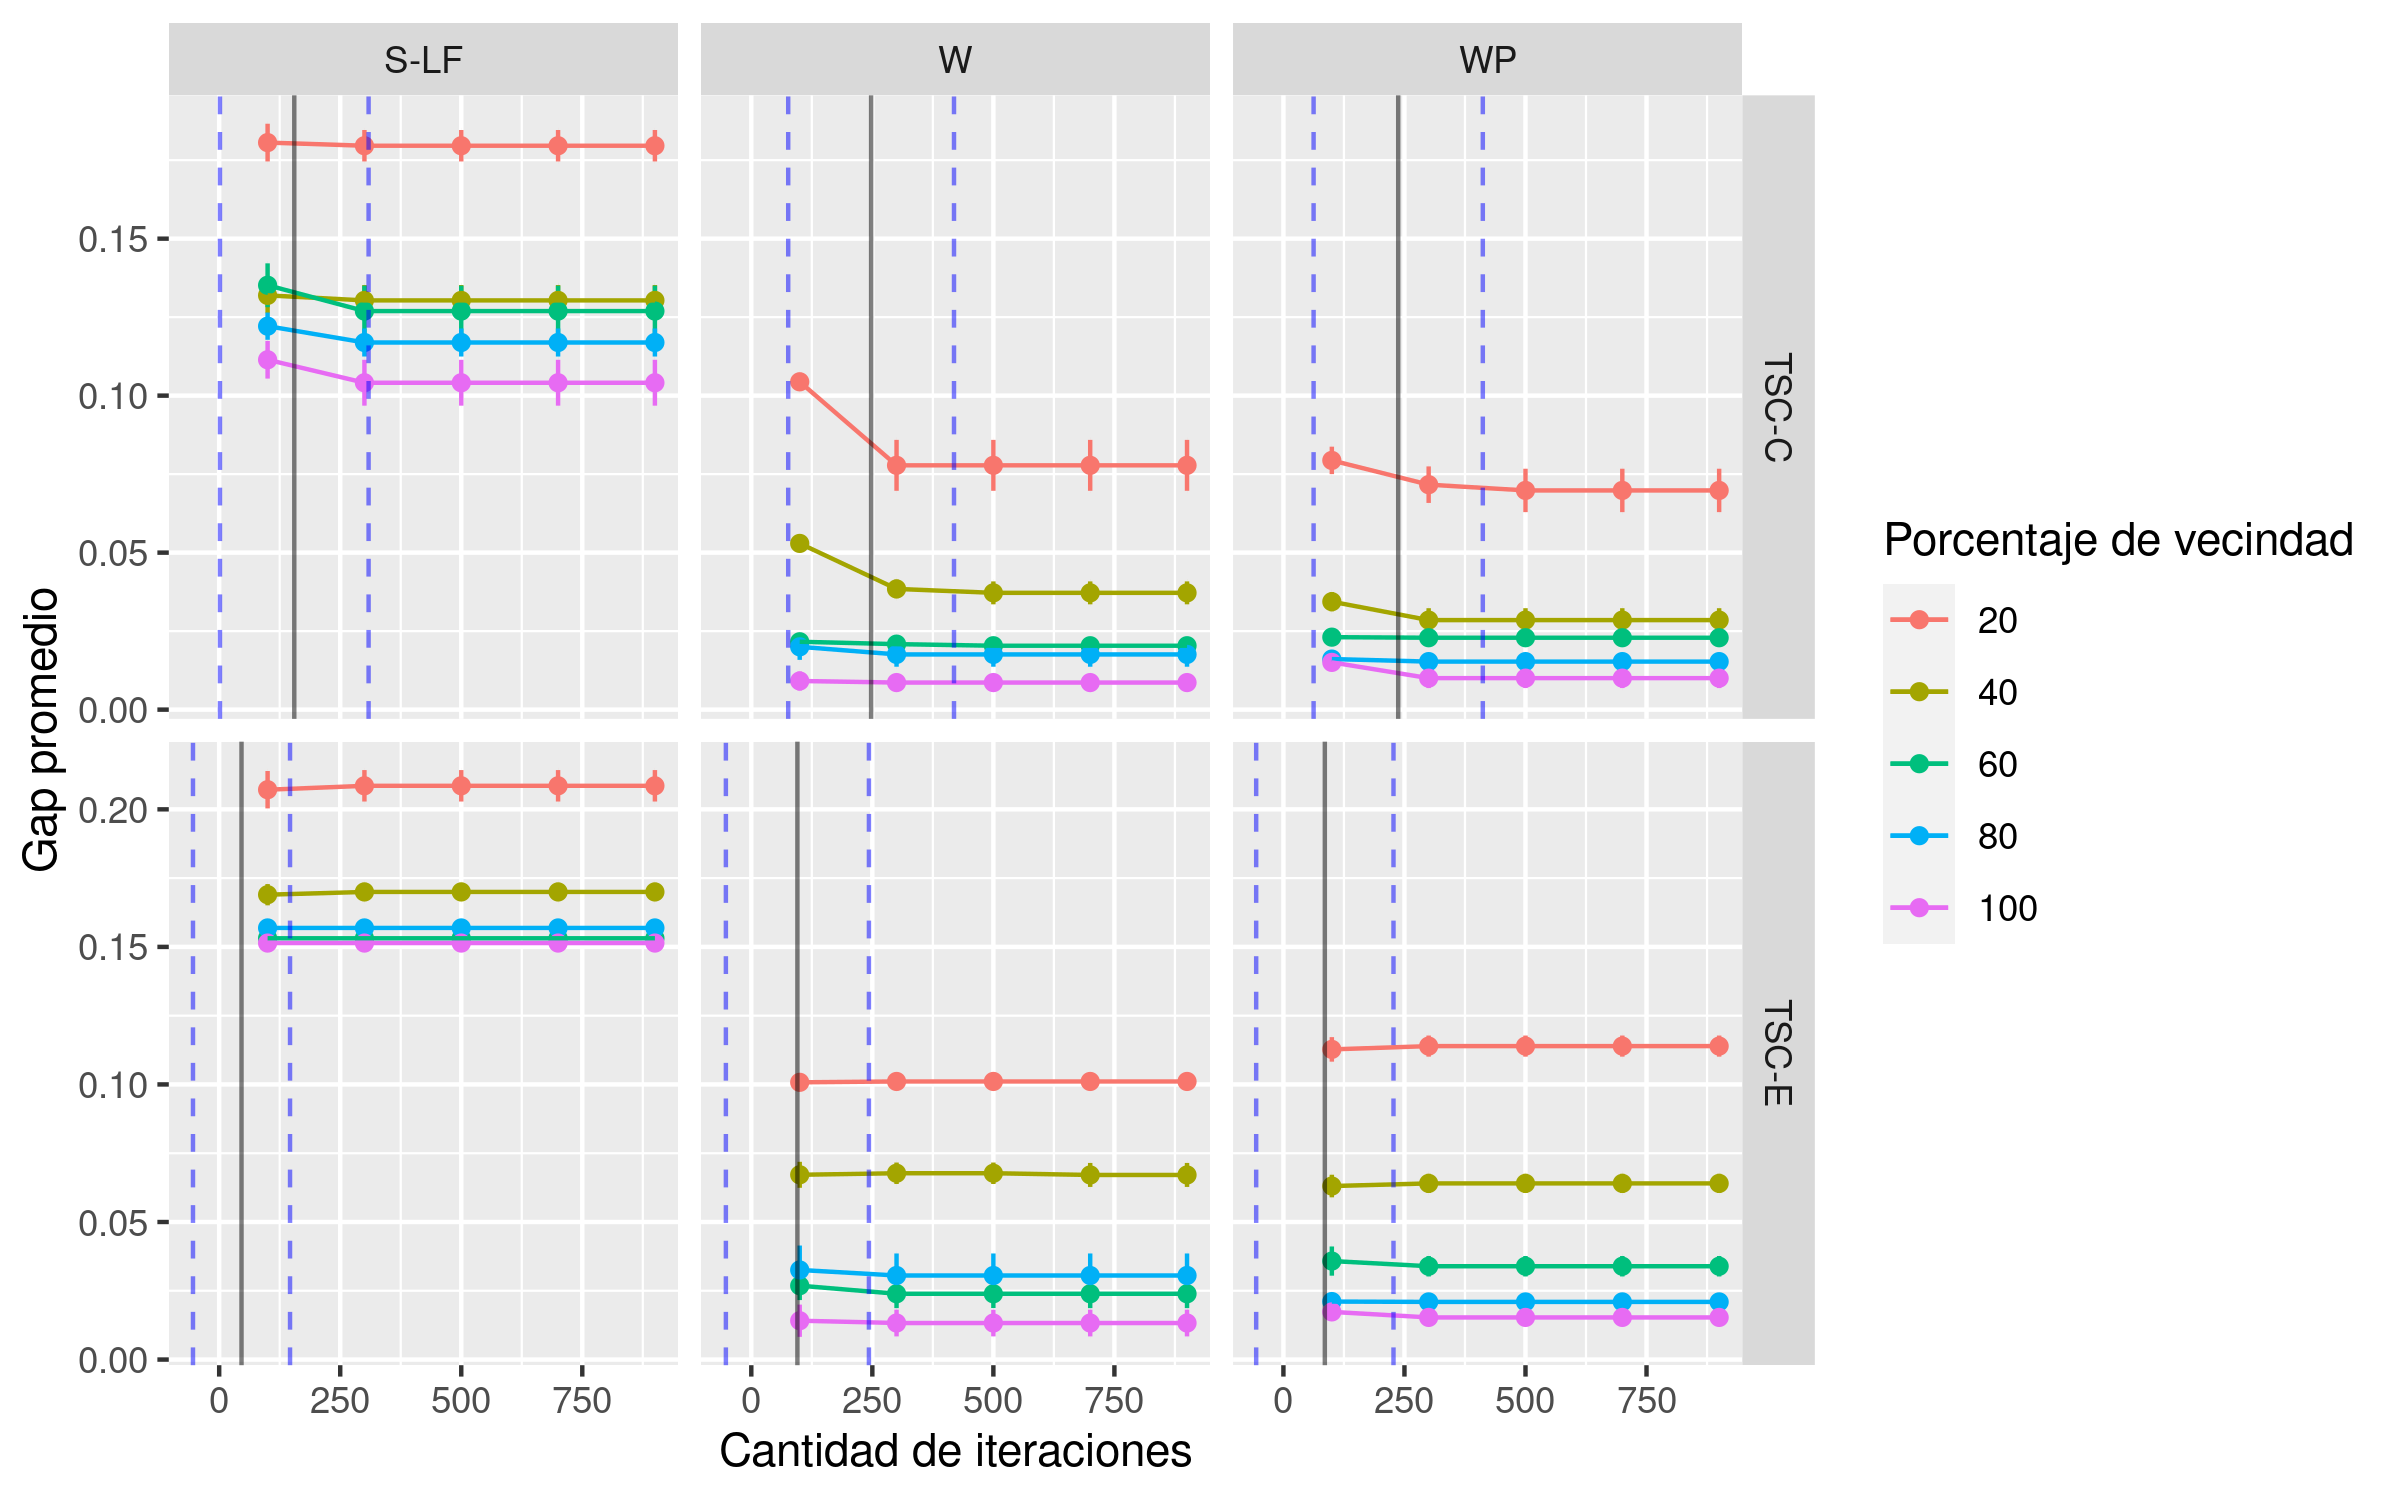
\includegraphics[width=0.8\textwidth]{plots/iteraciones_tsc.png}
    \caption{Se observa el gap promedio en función de la cantidad de memoria para todas las combinaciones de tabú search change y los algoritmos heurísticos iniciales. En todos los casos, se grafican los resultados obtenidos para valores de porcentaje de vecindad en [5, 20, 40, 60, 80, 100]. Se realizaron 5 repeticiones por instancia.}
    \label{plot:iteraciones tsc}
\end{figure}

\begin{figure}[H]
    \centering
    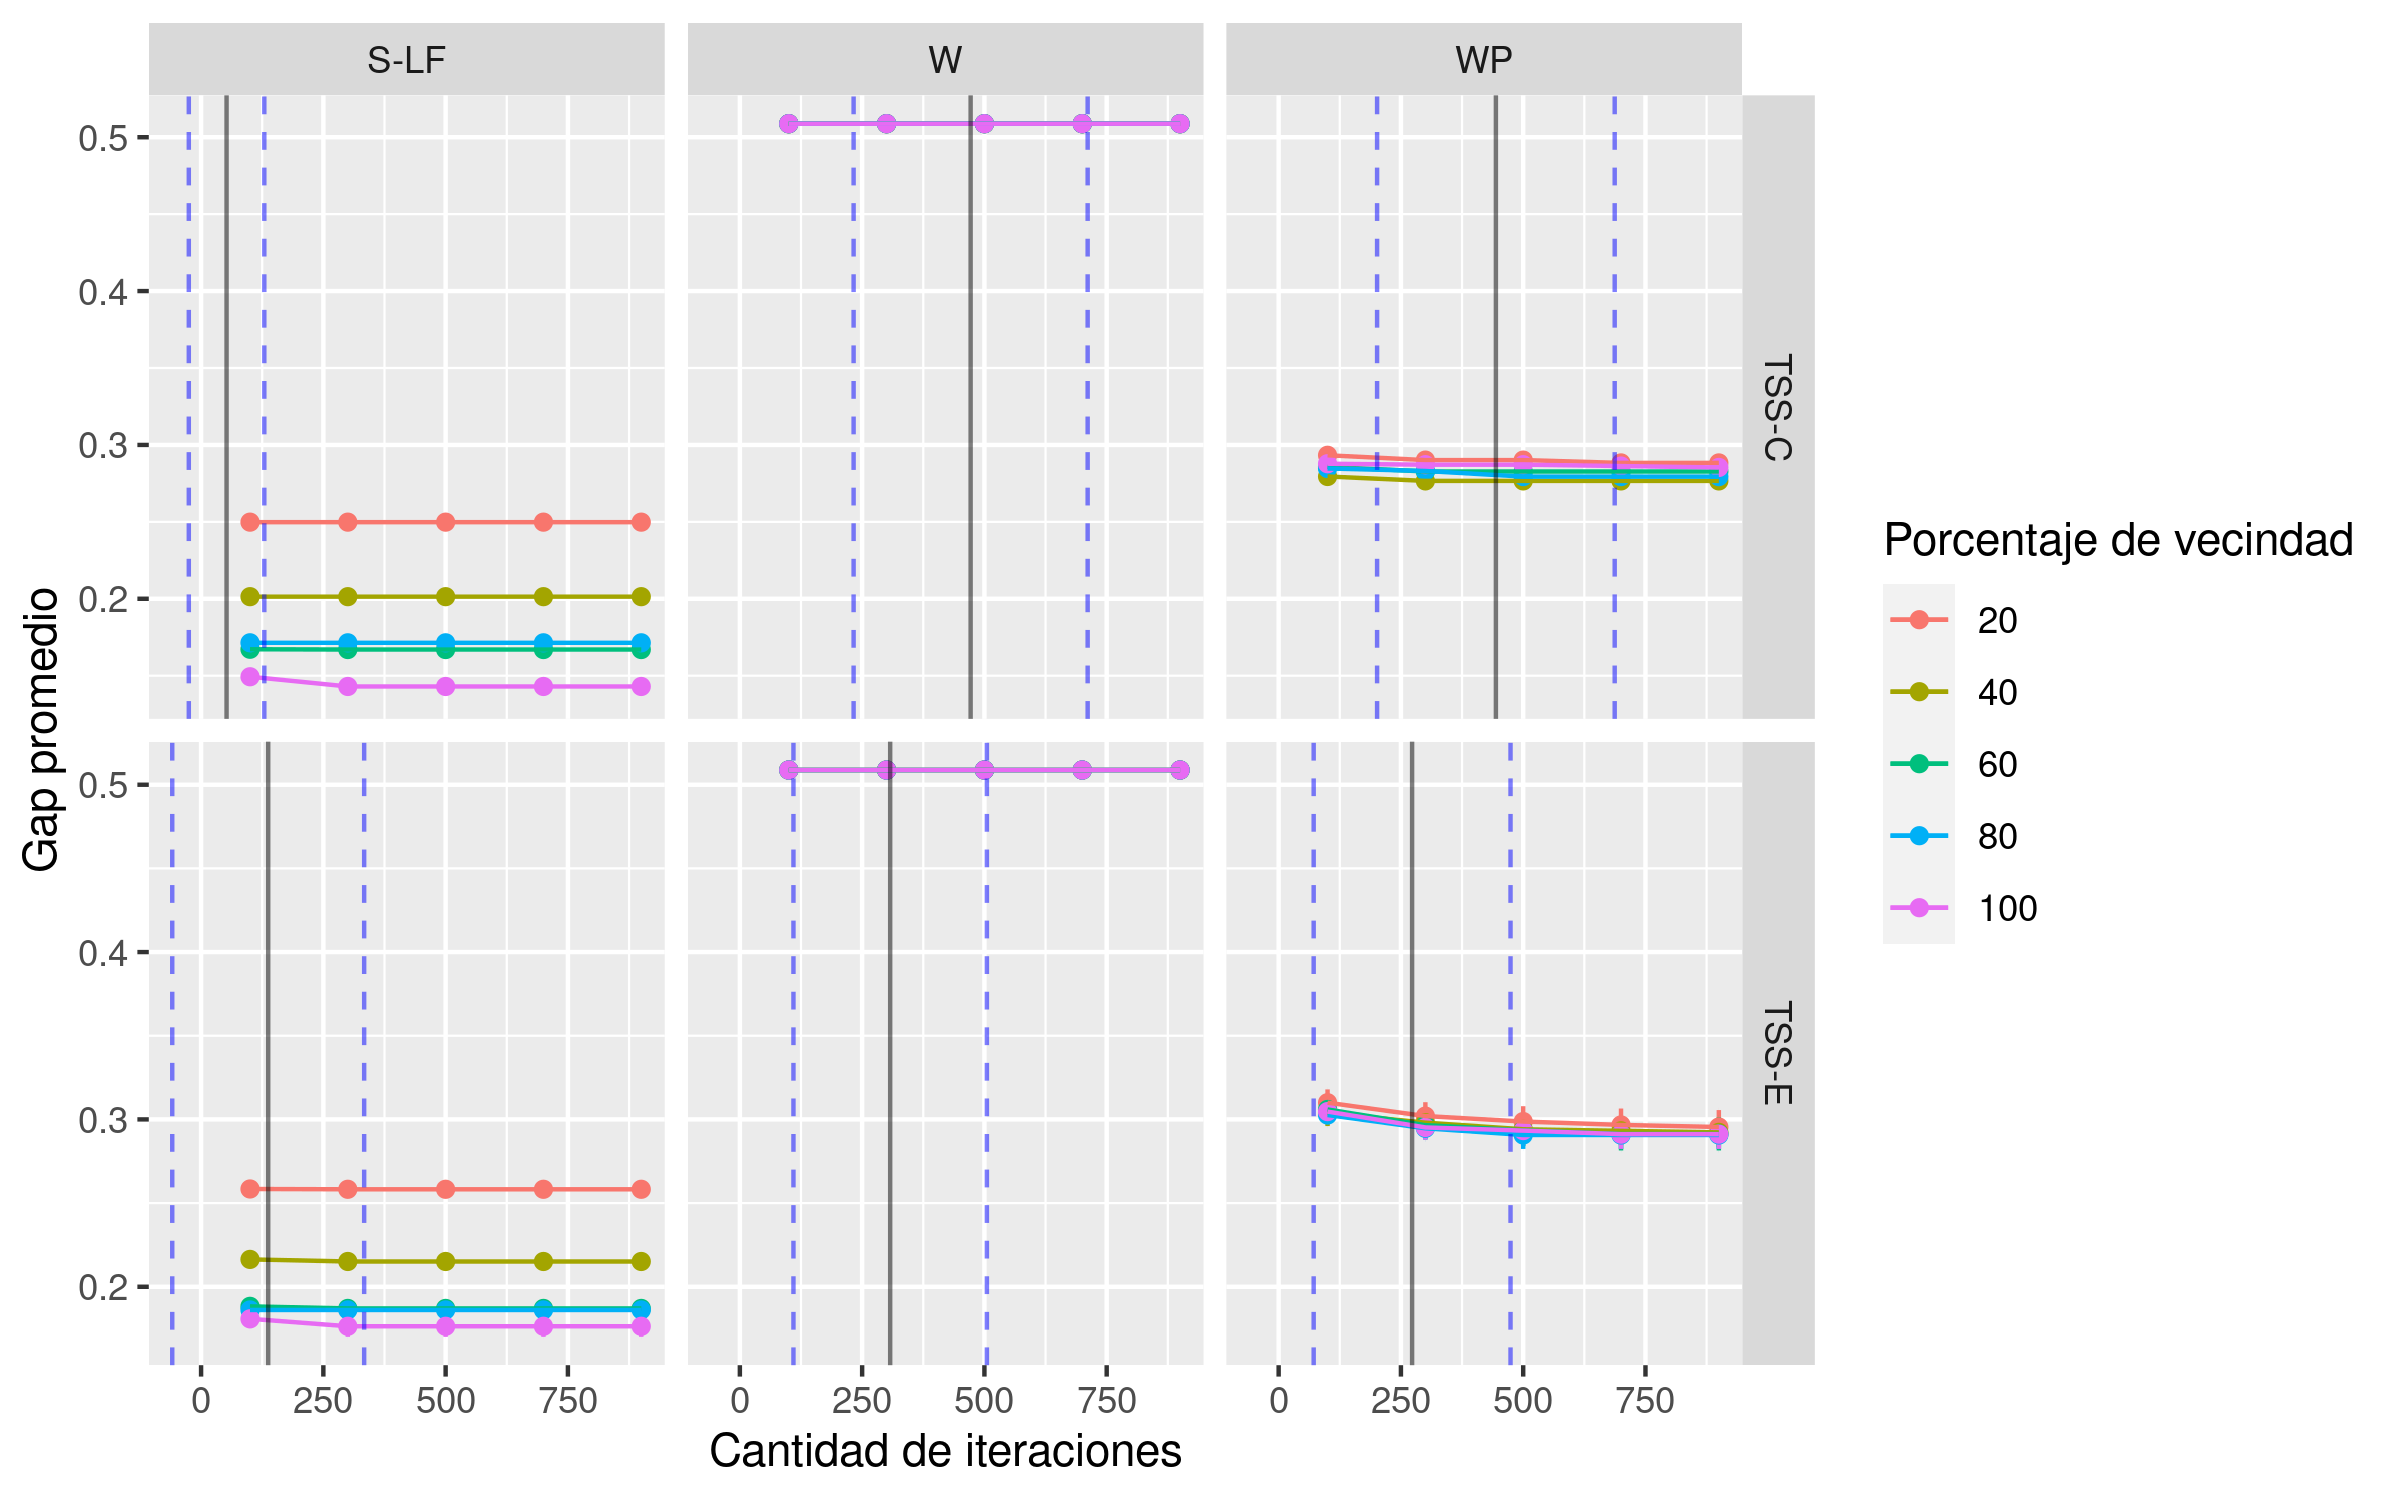
\includegraphics[width=0.8\textwidth]{plots/iteraciones_tss.png}
    \caption{Se observa el gap promedio en función de la cantidad de memoria para todas las combinaciones de tabú search swap y los algoritmos heurísticos iniciales. En todos los casos, se grafican los resultados obtenidos para valores de porcentaje de vecindad en [5, 20, 40, 60, 80, 100]. Se realizaron 5 repeticiones por instancia.}
    \label{plot:iteraciones tss}
\end{figure}

Considerando está sección y la anterior, ahora resulta más claro por qué había muchas combinaciones de parámetros que dan el mismo resultado en las Figura~\ref{plot:histogramas}. En general, se puede concluir que corridas con alta memoria o altas iteraciones terminan siendo equivalentes a las corridas que tienen valores cercanos a la cantidad de iteraciones efectivas.


\subsection{Evaluación}

Finalmente, para cada combinación de Tabú y heurística constructiva inicial, se eligieron las combinaciones que dieron mejor Gap en el set de datos de entrenamiento. En caso de que más de una configuración de parámetros diera resultados equivalentes se desempató por el tiempo de ejecución. Se detallan en la Tabla~\ref{tabla:ranking}.

En lineas generales no se observó correlación entre el tiempo de ejecución y la calidad de las soluciones entre los diferentes algoritmos de \textit{Tabú Search}. Esto puede observarse más en detalle en la fig. \ref{plot:correlacion gap tiempo}

Se puede observar que hay al menos un orden de magnitud de diferencia entre TSC usando heurística W o WP y el resto de los algoritmos, por lo que S-LF resulta la peor heurística constructiva para los TSC pero la mejor para los TSS por lo que explicado en la Sección 6.5. A su vez, notar que para TSC-E WP el número de iteraciones que da el mejor resultado es alto pero la diferencia en tiempo con las corridas que dan el resultado óptimo es muy chica, por lo que haber elegido ésta puede ser resultado de fluctuaciones experimentales. Sería interesante aumentar la cantidad de repeticiones y ver si se sigue eligiendo esta combinación de parámetros.

Por último, pareciera ser que la elección de estructura de Memoria no afecta el gap de TSS (salvo cuando usa S-LF porque tiene más posibilidades de encontrar mejorías), sólo el costo temporal. Aquí se confirma una vez más la importancia e injerencia del algoritmo inicial elegido en el desempeño del \textit{Tabú Swap}.

\begin{table}[ht]
\centering
\begin{tabular}{p{.5cm}p{1.5cm}p{1.8cm}p{1.8cm}p{2cm}p{1.8cm}p{1cm}p{1cm}p{1cm}}
  \hline
 & Variante de tabu & Heurística Inicial & Iteraciones & Porcentaje de Vecindad & Cantidad de Memoria & Aspirar & Gap medio & Tiempo medio (s) \\ 
  \hline
1 & TSC-C & WP & 300 & 90 & 100 & Si & 0 & 4.50 \\ 
  2 & TSC-E & W & 100 & 90 & 35 & Si & 0.003 & 1.04 \\ 
  3 & TSC-C & W & 300 & 50 & 50 & No & 0.003 & 3.35 \\ 
  4 & TSC-E & WP & 900 & 100 & 50 & Si & 0.009 & 0.80 \\ 
  5 & TSC-C & S-LF & 300 & 100 & 50 & Si & 0.089 & 2.68 \\ 
  6 & TSC-E & S-LF & 300 & 70 & 35 & Si & 0.131 & 0.34 \\ 
  7 & TSS-C & S-LF & 300 & 100 & 50 & No & 0.137 & 3.37 \\ 
  8 & TSS-E & S-LF & 300 & 100 & 100 & Si & 0.154 & 4.47 \\ 
  9 & TSS-E & WP & 500 & 60 & 100 & Si & 0.271 & 10.56 \\ 
  10 & TSS-C & WP & 700 & 25 & 35 & Si & 0.271 & 15.29 \\ 
  11 & TSS-E & W & 100 & 5 & 20 & No & 0.509 & 1.85 \\ 
  12 & TSS-C & W & 100 & 5 & 20 & Si & 0.509 & 2.20 \\ 
   \hline
\end{tabular}
\caption{Cuadro comparativo que presenta la mejor combinación de metaparámetros para cada algoritmo evaluado (combinación de tabú search y heurísticas iniciales). Se ordenan las entradas según el valor de gap promedio obtenido.}
\label{tabla:ranking}
\end{table}

Para analizar el desempeño de los algoritmos en instancias de testeo y evitar así cualquier tipo de \textit{overfitting} se corrió cada combinación de algoritmo tabú con inicial, utilizando los parámetros óptimos encontrados en el entrenamieinito. Los resultados se detallan en la Figura~\ref{plot:ranking}.

\begin{figure}[H]
    \centering
    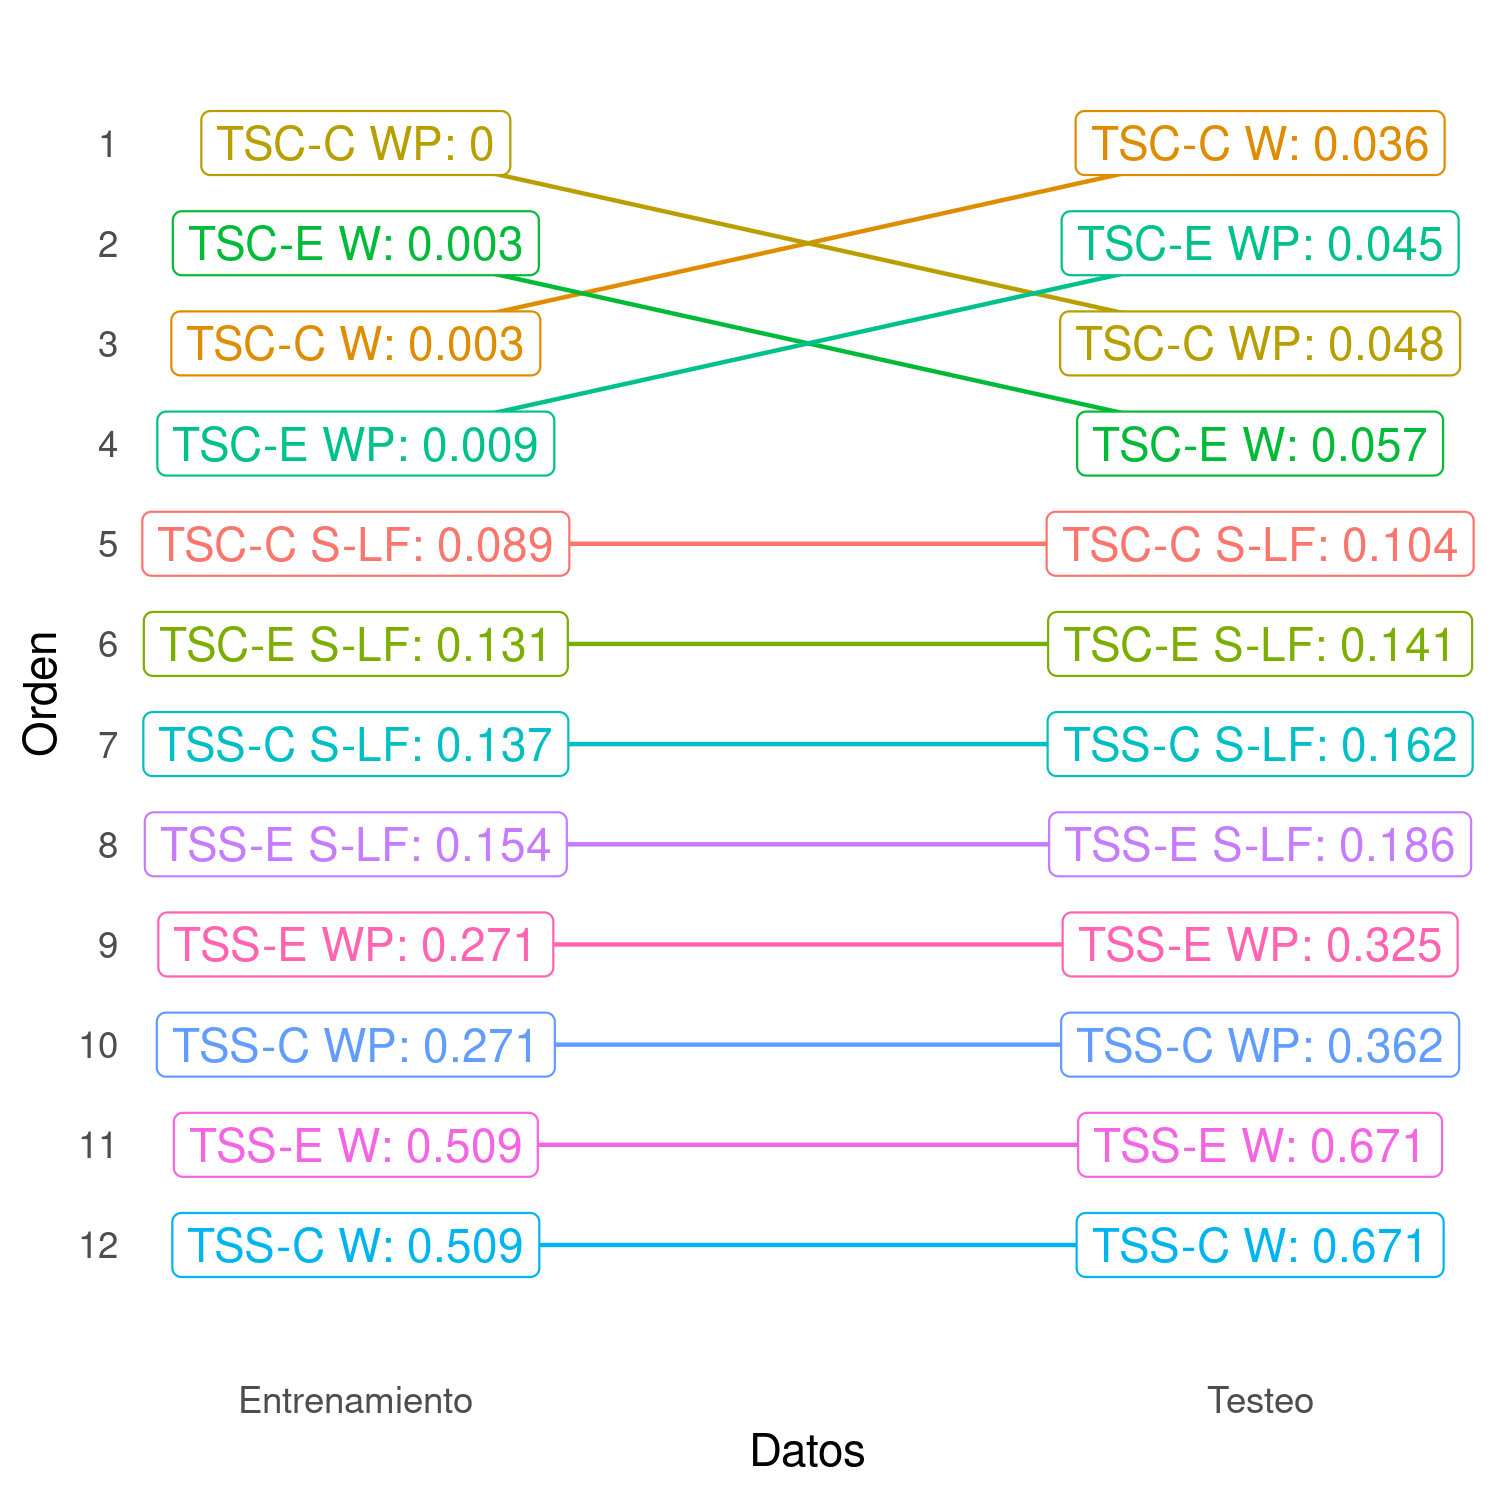
\includegraphics[scale = 0.7]{plots/ranking.png}
    \caption{Se observa el orden o ranking de algoritmos según los valores obtenidos de gap medio. A la izquierda se observa el ranking calculado para las instancias de entrenamiento, mientras que a la derecha, para las instancias de testeo.}
    \label{plot:ranking}
\end{figure}

Los resultados con el set de datos de testeo son peores, lo cual es esperable pero podría estar indicando \textit{overfitting} en el entrenamiento, sobre todo para TSC-C WP que da gap 0 en las instancias de entrenamiento. Sin embargo, se mantiene la diferencia de al menos un orden de magnitud entre TSC usando heurística W o WP y el resto de los algoritmos, por lo que el orden de eficiencia de los algoritmos se mantiene.